%##############################################################################
% Preambu³a dokumentu
% 17.12.2010
%
\documentclass[12pt,a4paper,twoside
%,draft%<------------------- opcja "draft" tylko markuje rysunki w tekscie
]{report}
\usepackage{graphicx}
\usepackage[pdftex]{hyperref}
\usepackage{breakurl}
\usepackage{polski}
\usepackage[utf8]{inputenc}
%\usepackage[cp1250]{inputenc}%<------------ strona kodowa dla MSWindows
\usepackage{t1enc,amsmath}
\usepackage{times,caption}
\usepackage{bsc_pl}
\usepackage{fancyhdr}%<-------------------- formatowanie nag³ówka i stopki
\usepackage{float}

% ustawienia obrazow %
\graphicspath{ {./assets/} }
\DeclareGraphicsExtensions{.pdf,.png,.jpg}

\linespread{1.5}

\pagestyle{fancy}%<--------------- styl z fancyhdr.sty; definicje nag³ówka
%-----------------------------------------------------------------------
% Definicje nag³ówka dostêpne z pakietem fancy.sty
\renewcommand{\headheight}{15pt}%<---------------- szerokoœæ nag³owka
\renewcommand{\headrulewidth}{0.4pt}%<------------ gruboœæ linii w nag³ówku
\fancyhead[RO,LE]{\thepage}
\fancyhead[LO]{\footnotesize \slshape \rightmark}%  <- mniejsze litery w tytule sekcji
\fancyhead[RE]{\footnotesize \slshape \leftmark}%   <-- i nag³ówka
\cfoot{}%<---------------------------------- likwidacja numerów w stopce
%-------------------------------------------------------------------------
\newcommand*{\mbf}{\mathbf}
\newcommand*{\bs}{\boldsymbol}
%
%\renewcommand*\captionlabeldelim{.}
\renewcommand{\captionlabelfont}{\bfseries}
\renewcommand{\captionsize}{\small}
%
% Koniec preambu³y
%##############################################################################
%
% Pocz¹tek w³aœciwego dokumentu
%
\begin{document}
%
\bibliographystyle{unsrt} % <- Ustawienie stylu bibliografi (unsrt,abbrv)
%<------------------------------------------ 
% Dane do strony tytu³owej
% Zmieniæ argumenty poleceñ: \author, \title i \graduationdate
%
\author{Imię i Nazwisko} 
\title{Tytuł pracy}
\graduationdate{Gliwice, styczeń 2013}
%<------------------------------------------
% Tworzona strona tytu³owa 
\titlepage 
\thispagestyle{empty}%<--------------------- pusta strona na odwrocie tutu³owej
\cleardoublepage%<-------------------------- dalej bêdzie od nieparzystej
%<------------------------------------------
% Tworzony spis treœci
\renewcommand*{\baselinestretch}{0.8}
\tableofcontents
\newpage
\thispagestyle{empty}
\cleardoublepage
\renewcommand*{\baselinestretch}{1.0}
%-------------------------------------------------------------------------------
% Wstawianie wykazu oznaczeñ
\addcontentsline{toc}{chapter}{Wykaz ważniejszych oznaczeń} % <-----  Je¿eli w 
% dokumencie nie ma wykazu oznaczeñ, nale¿y wykomentowaæ t¹ liniê
%\chapter*{Wykaz wa�niejszych oznacze�}
{\small
\begin{tabular}{ccp{10cm}}
  $\bf{A}$ & -- & magnetyczny potencja� wektorowy\\
  $AF$ & -- & charakterystyka grupowa dyskretnego uk�adu antenowego\\
  $A,~B$ & -- & funkcja\\
  $c$ & -- & pr�dko�� �wiat�a w~pr�ni\\
  $d$ & -- & wysoko�� modu�u anteny, odleg�o�� pomi�dzy �r�d�ami modelu dyskretnego\\
  $D$ & -- & najwi�kszy wymiar liniowy anteny\\
  $\bf{D}$ & -- & wsp�czynnik dyfrakcji\\
  ${\bf E}$ & -- & zespolony wektor nat�enia pola elektrycznego\\
  ${\bf E}_i$ & -- & sk�adowa indukcyjna pola elektrycznego\\
  ${\bf E}_p$ & -- & sk�adowa promieniowania pola elektrycznego\\
  $E$ & -- & warto�� skuteczna nat�enia pola elektrycznego\\
  ${\bf E}^p$ & -- & sk�adowa elektryczna pola pierwotnego\\
  ${\bf E}^w$ & -- & sk�adowa elektryczna pola wt�rnego\\
  $e$ & -- & podstawa logarytmu naturalnego \\
  $\bf{F}$ & -- & elektryczny potencja� wektorowy\\
  $F$ & -- & ca�ka Fresnela\\
  $f$ & -- & cz�stotliwo��, funkcja\\
  $[F],~[G]$ & -- & wektor kolumnowy\\
  F/B & -- & stosunek promieniowania prz�d/ty�\\
  $F_{\: \rm m}(\theta,\phi)$ & -- &
  charakterystyka promieniowania odosobnionego modu�u
  anteny dla pola elektrycznego\\
  $F_{\: \rm V}(\theta)$ & -- &
  charakterystyka promieniowania odosobnionego modu�u
  anteny w~p�a\-szczy\-�nie pionowej\\
  $F_{\: \rm H}(\phi)$ & -- &
  charakterystyka promieniowania odosobnionego modu�u
  anteny w~p�a\-szczy\-�nie poziomej\\
  $g$ & -- & funkcja\\
  $G(\phi, \theta)$ & -- & funkcja zysku energetycznego anteny\\
  $G$ & -- & zysk energetyczny\\
  $G_c(\phi)$ & -- & funkcja zysku energetycznego dla fali cylindrycznej\\
  $G_c$ & -- & zysk energetyczny �r�d�a fali cylindrycznej\\
  $g_{\rm H}(\phi)$ & -- & charakterystyka promieniowania mocy w~p�a\-szczy\-�nie poziomej\\
  $G_{\rm m}(\phi, \theta)$ & -- & funkcja zysku energetycznego odosobnionego modu�u anteny
      \end{tabular}
} \newpage  \thispagestyle{empty}
 {\small
\begin{tabular}{lcp{9cm}}
  $G_{\rm m}$ & -- & zysk energetyczny odosobnionego modu�u anteny\\
  $h$ & -- & wysoko�� anteny\\
  $\bf{H}$ & -- & zespolony wektor nat�enia pola magnetycznego\\
  $\bf{H}_i$ & -- & sk�adowa indukcyjna pola magnetycznego\\
  $\bf{H}_p$ & -- & sk�adowa promieniowania pola magnetycznego\\
  $H$ & -- & warto�� skuteczna nat�enia pola magnetycznego\\
  ${\bf H}^p$ & -- & sk�adowa magnetyczna pola pierwotnego\\
  ${\bf H}^w$ & -- & sk�adowa magnetyczna pola wt�rnego\\
  $[I]$ & -- & wektor pr�du \\
  $j$ & -- & jednostka urojona \\
  $k$ & -- & liczba falowa \\
  ${\bf J}_s$ & -- & g�sto�� elektrycznego pr�du powierzchniowego\\
  $[L]$ & -- & macierz kwadratowa\\
  $L$ & -- & operator liniowy\\
  $l$ & -- & d�ugo��\\
  ${\bf M}_s$ & -- & g�sto�� magnetycznego pr�du powierzchniowego\\
  $P$ & -- & moc wypromieniowana przez anten�\\
  ${\bf r}$ & -- & wektor wodz�cy \\
  $r_{\rm d}$ & -- & granica obszaru pola dalekiego odosobnionego
  modu�u anteny\\
  $R,~r$ & -- & odleg�o��\\
  $R$ & -- & wsp�czynnik odbicia \\
  $\bf{S}$ & -- & zespolony wektor g�sto�ci strumienia mocy\\
  $S_c$ & -- & warto�� �rednia g�sto�ci strumienia mocy fali cylindrycznej\\
  $\bf{S}_p$ & -- & wektor g�sto�ci strumienia mocy skojarzony z~polem promieniowania\\
  $S$ & -- & warto�� �rednia g�sto�ci strumienia mocy\\
  $s$ & -- & odleg�o�� \\
  SAR & -- & tempo poch�aniania na jednostk� masy\\
  $T$ & -- & wsp�czynnik transmisji\\
  $u$ & -- & funkcja, pr�dko�� rozchodzenia si� fali w~o�rodku\\
  $[V]$ & -- & wektor pobudzenia \\
  $w$ & -- & szeroko�� anteny\\
  $w_n$ & -- & $n$-ta funkcja wagowa\\
  $x,~y,~z,$ & -- & wsp�rz�dne prostok�tne punktu \\
  $[Z]$ & -- & macierz impedancyjna tworzona metod� moment�w \\
  ${\bf 1}_{p}$ & -- & wektor jednostkowy okre�laj�cy polaryzacj� pola \\%wytwarzanego przez $i$-te �r�d�o\\
  $\nabla$ & -- & operator nabla\\
  $\alpha$ & -- & t�umienno�� o�rodka\\
  $\alpha_n$ & -- & $n$-ty wsp�czynnik rozwini�cia\\
  $\Delta x$ & -- & krok dyskretyzacji przestrzeni\\
  $\Delta t$ & -- & krok dyskretyzacji czasu\\
  $\epsilon$ & -- & przenikalno�� elektryczna \\
  $\varepsilon$ & -- & b��d wzgl�dny
 \end{tabular}
}
\newpage
\thispagestyle{empty}%<---------------------------- pusta strona na odwrocie tutu�owej
%\pagestyle{fancy}
\cleardoublepage%<--------------------------------- dalej b�dzie od nieparzystej

%-------------------------------------------------------------------------------
% Wstawiane poszczególne rozdzia³y pracy
%

\singlespacing
\chapter{Wstęp}

\section{Od kodu kreskowego do tagu radiowego}

Obserwujemy na przestrzeni ostatnich kulkudziesieciu lat znaczący rozwój technologii bezprzewodowej oraz mobilnych form płatności elektronicznej spowodował, że obecnie niemal na każdym kroku spotykamy się z systemami automatycznej identyfikacji (ang. \emph{Auto ID Systems}). Systemy te umożliwiają szybką, wygodną i bezbłędną identyfikacje produktów, sprzętu, ludzi a nawet zwierząt. Przekłada się to zazwyczaj na poprawę poziomu życia oraz jakości świadczonych usług spedycyjnych. Podstawowym zadaniem systemów automatycznej identyfikacji jest sprawne, przeprowadzone w czasie rzeczywistym i bez udziału człowieka, zarządzanie łańcuchem dostaw oraz kontrola jednostek logistycznych. Ostatnio systemy te coraz częściej wykorzystuje się do autoryzacji transakcji bankowych realizowanych za pośrednictwem sieci telefonii komórkowej, sieci przewodowej LAN i bezprzewodowej WLAN.


\noindent 
\newline Systemy automatycznej identyfikacji obejmują:
\begin{itemize}\setlength{\itemsep}{0pt}
    \item systemy kodów kreskoweych (ang. \emph{bar code}),
    \item systemy kart elektronicznych (ang. \emph{electronic cards}),ścieżki magnetyczne (ang. \emph{magnetic stripe}),
    \item systemy RFID (ang. \emph{Radio Frequency Identyfication}),
    \item systemy automatycznego rozpoznawania pisma ręcznego ICR (ang. \emph{Intelligent Charakter Recognition}), 
    \item systemy automatycznego rozpoznawanie znaków (druku) OCR (ang. \emph{Optical Character Recognition}),
    \item systemy biometryczne bazujące na technice:
	\begin{itemize}\setlength{\itemsep}{0pt}
		\item identyfikacji linii papilarnych,
		\item identyfikacji głosu,
		\item identyfikacji siatkówki oka,
		\item rozpoznawaniu twarzy
	\end{itemize}
\end{itemize}

Za protoplastę systemów automatycznej identyfikacji zwykło się uważać systemy kodów kreskowych, wprowadzone do powszechnego użytkuw latach 60-tych XX wieku.
Kod kreskowy nazywany często potocznie kodem paskowym (ang. \emph{bar code}) stanowi szereg ciemnych i jasnych pasków o zróżnicowanej szerokości wykorzystywanych do zakodowania danych cyfrowych. Wykorzystując własności statyczne nośnika informacji, w tym przypadku białej i czarnej farby tworzącej pasek kodu kreskowego, jesteśmy w stanie szybko i w sposób jednoznaczny dokonać identyfikacyji skanowanego obiektu. Emitowane przez czytnik światło zostaje odbite od jasnych pasków, a pochłonięte przez paski czarne. Dekodowanie informacji cyfrowej zapisanej w kodzie kreskowym sprowadza się do porównania, mierzonego w luksach, natężenia światła emitowanego przez czytnik z natężeniem światła dbitym przez kod kreskowy. Zastosowanie odpowiedniego fotodetektora pozwala różnicę w poziomie natężenia światła przekształcić w ciąg impulsów elektrycznych, które są następnie przesyłane do komputera. W komputerze impulsy te są przetwarzane na ciąg odpowiednich znaków alfanumerycznych zapisywanych w bazie danych. 
Kody kreskowe są powszechnym i tanim sposobem etykietowania produktów. Zaletą tego systemu jest powszechna unifikacja sposobu kodowania. Wadami  natomiast możliwość zapisu małej ilości danych  oraz częsty problem z ich odczytem (dane trzeba wprowadzać ręcznie). Duży problem w wielu sytuacjach stanowi również niewielka dopuszczalna odległość kodu od czytnika. 
Technologia kodów kreskowych jest obecnie najbardziej rozpowszechnioną i najtańszą technologią znakowania produktów, jednak osiągnęła już swoje granice możliwości – w pewnych zastosowaniach jest już niewystarczająca.
Coraz większą popularność zyskuje technika identyfikacji radiowej – \emph{RFID}. System jest bardzo prosty dzięki temu zyskuje na popularności zarówno przy dużych i kosztownych projektach jak również  niewielkich przedsięwzięciach.

\section{Struktura systemu \emph{RFID}}

RFID (ang.\emph {Radio Frequency  Identyfication}) to jedna z najszybciej rozwijających  się automatycznych technologii bezprzewodowej  identyfikacji. Technologia ta umożliwia zdalne przechowywanie i odczytywanie danych z układów nazywanych znacznikami (ang. \emph{tag}) za pośrednictwiem fal radiowych. 

\noindent  
\newline W skład typowego systemu \emph{RFID} wchodzą następujące podzespoły:
\begin{itemize}\setlength{\itemsep}{0pt}

	\item znacznik  (etykieta, transponder, tag) –zbudowany z układu elektronicznego najczęściej microchipa z pamięcią, w którym dane są  kodowane i zapisywane w pamięci podręcznej oraz transmitowane za pomocą anteny nadawczo-odbiorczej (często napylanej na warstwie izolatora). Układ identyfikatora wykonany jest zazwyczaj na podłożu z papieru lub plastiku. 

	Etykiety \emph{RFID} mogą zawierać zarówno informacje zapisane w formie elektronicznej (pod postacią danych) jak również naniesiony tekst lub kod kreskowy. 

	Identyfikatory możemy sklasyfikować na dwa sposoby. W zależności od sposobu zasilania i sposobu zapisu danych. 

	\item czytnik - zbudowany z mikrokomputera, który weryfikuje poprawność otrzymanych informacji, modułu transmisji radiowej czyli nadajnika i odbiornika  odpowiedzialnych za odczyt i zapis danych w identyfikatorze oraz anteny lub cewki. Niektóre czytniki posiadają dodatkowo interfejs łączący z komputerem \emph{PC} (pozwalający na transmisję danych pomiędzy czytnikiem a komputerem).
	
	Oprogramowanie czytnika składa się z warstwy komunikacyjnej i użytkowej. Warstwa komunikacyjna odpowiedzialna jest za techniczną stronę transmisji danych, a warstwa użytkowa odpowiada za poprawne działanie aplikacji czyli wymianę, gromadzenię i przetwarzanie informacji na serwerze lub aplikacji klienckiej.


\end{itemize}



\section{Kryteria podziału znaczników i czytników}

\noindent 
Ze względu na sposób zasilania znaczniki dzielimy na: 
\begin{itemize}\setlength{\itemsep}{0pt}

	\item pasywne  (ang. \emph{passive}) (bez wewnętrznego zasilania) do zasilania  wykorzystują energię pozyskaną z pola elektromagnetycznego wytwarzonego przez czytnik, stanowią obecnie grupę najliczniej eksploatowanych znaczników, 

	\item aktywne (ang. \emph{active}) (z własnym źródłem zasilania np. baterią), emitują wiekszy poziom mocy sygnału zwrotnego, pracują zazwyczaj na większych częstotliwościach przez co transmisja danych trwa krócej niż w innych znacznikach. Stosuje się je przede wszystkim do identyfikacji pojazdów,
	
	\item pół-pasywne (ang. \emph{semi-passive}) łączą cechy zarówno transponderów aktywnych jak i pasywnych. Transpondery te wyposażone są w baterię, która zasila obwód elektroniczny. Zasięg odczytu sięga 100 m, w dużym stopniu jednak zależy od czułości odbiornika w czytniku.  

\end{itemize}

\noindent 
\newline Ze względu na sposób zapisu danych znaczniki dzielimy na:
\begin{itemize}\setlength{\itemsep}{0pt}

	\item znaczniki typu \emph{RO} (ang.\emph{read only}) - tylko do odczytu – programowane podczas produkcji, zawierają numer seryjny (mogą zawierać również inne dane, których nie można modyfikować), 

	\item znaczniki typu \emph{RW} (ang.\emph{read write}) - do wielokrotnego zapisu i odczytu – zapisane dane mogą być wielokrotnie modyfikowane (pamięć może być podzielona na dwie części: część tylko do odczytu i część w której użytkownik może modyfikować zapisane dane),

	\item znaczniki typu\emph{WORM} (ang.\emph{write once read many}) - do jednokrotnego zapisu i wielokrotnego odczytu, część danych zapisana jest trwale, a część może być zmieniona przez użytkownika.

\end{itemize}


\noindent 
\newline Klasyfikacji czytników można dokonać według dwóch kryteriów - kryterium mobilności i kryterium komunikacji.



\noindent 
\newline Ze względu na na kryterium mobilności czytniki dzielimy na:

\begin{itemize}\setlength{\itemsep}{0pt}

	\item stacjonarne - pracujące w trybie autonomicznym – cały czas sczytuje etykiety znajdujące się w jego zasięgu, 

	\item interaktywne – w tym trybie komunikacja odbywa się za pomocą aplikacji pracującej na serwerze lub aplikacji klienckiej, 

	\item ruchome, przenośne.
\end{itemize}




\noindent
\newline Ze względu na typu interfejsu komunikacyjnego czytniki dzielimy na:

\begin{itemize}\setlength{\itemsep}{0pt}

	\item szeregowe - porty RS-232 lub RS-485, 

	\item sieciowe z interfejsem sieciowym np. Ethernet.

\end{itemize}



Technologia \emph{RFID} w ostatnim dziesięcioleciu zyskała miano jednego z najbardziej obiecujących i najprężniej rozwijających się systemów identyfikacji.
System \emph{RFID} pozwala na dużą automatyzację pracy zarówno podczas zapisu jak i odczytu danych. W przeciwieństwie do kodów kreskowych technologia ta nie wymaga bezpośredniej "widoczności" pomiędzy etykietą, a czytnikiem oraz daje możliwość odczytu i przetwarzania wielu etykiet równocześnie.

%\newpage

\section{Zakresy częstotliwości}

Obecnie wdrażane systemy \emph{RFID} pracują na różnych zakresach częstotliwości, które można podzielić na następujące pasma:

\begin{itemize}\setlength{\itemsep}{0pt}
	\item pasmo niskich częstotliwości \emph {LF} (125-134.2 kHz).
Znaczniki \emph{LF} są zazwyczaj pasywne i wyróżniają się małą wrażliwością na obecność w pobliżu elementów metalowych, substancji płynnych oraz innych elementów wykonanych z dobrych przewodników. Powoduje to, że znaczniki tego typu świetnie sprawdzają się jako identyfikatory narzędzi, podzespołów maszyn, pojazdów czy metalowych kontenerów. Znalazły również zastosowanie w rolnictwie do oznakowania zwierząt, leków oraz produktów spożywczych, gdyż fale elektromagnetyczne o niskiej częstotliwości wnikają w tkanki ciała i płyny.
Wygląd i budowa znaczników \emph{LF} zależy ściśle od ich przeznaczenia. Znaczniki używane jako immobilizery (czyli elektroniczne zabezpieczenia przed niepowołanym uruchomieniem pojazdu) zazwyczaj wbudowane są w kluczyk natomiast cewka /  antena czytnika \emph{RFID} umieszczona jest współosiowo w stacyjce samochodu.
   
	\begin{figure}[h!]
	\centering
	    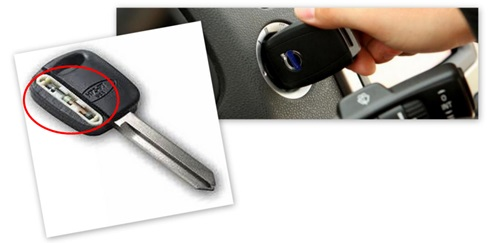
\includegraphics[width=9.32cm]{immobilizer.jpg}
	    \caption{Immobilizer samochodowy w technologii RFID}
	\end{figure}

	Dodatkowo systemy pracujące na częstotliwośći 135 kHz znalazły zastosowanie w automatycznej identyfikacji zwierząt hodowlanych i domowych.

	\begin{figure}[h!]
	\centering
	    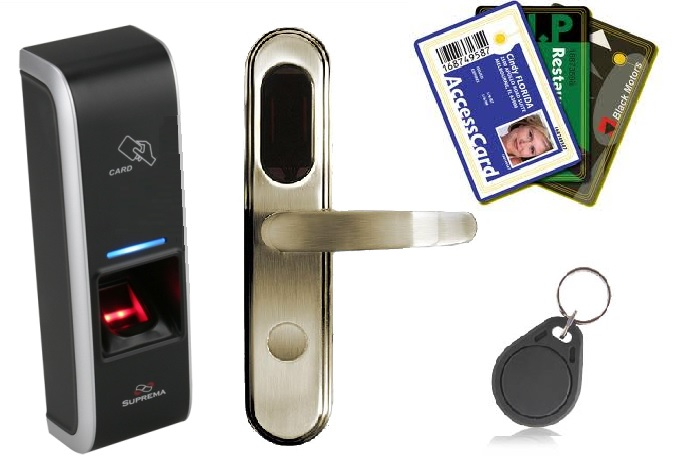
\includegraphics[width=7.27cm]{automatyczna_identyfikacja.jpg}
	    \caption{System kontroli dostępu bazujący na technologii RFID}
	\end{figure}
	
	\begin{figure}[h!]
	\centering
	    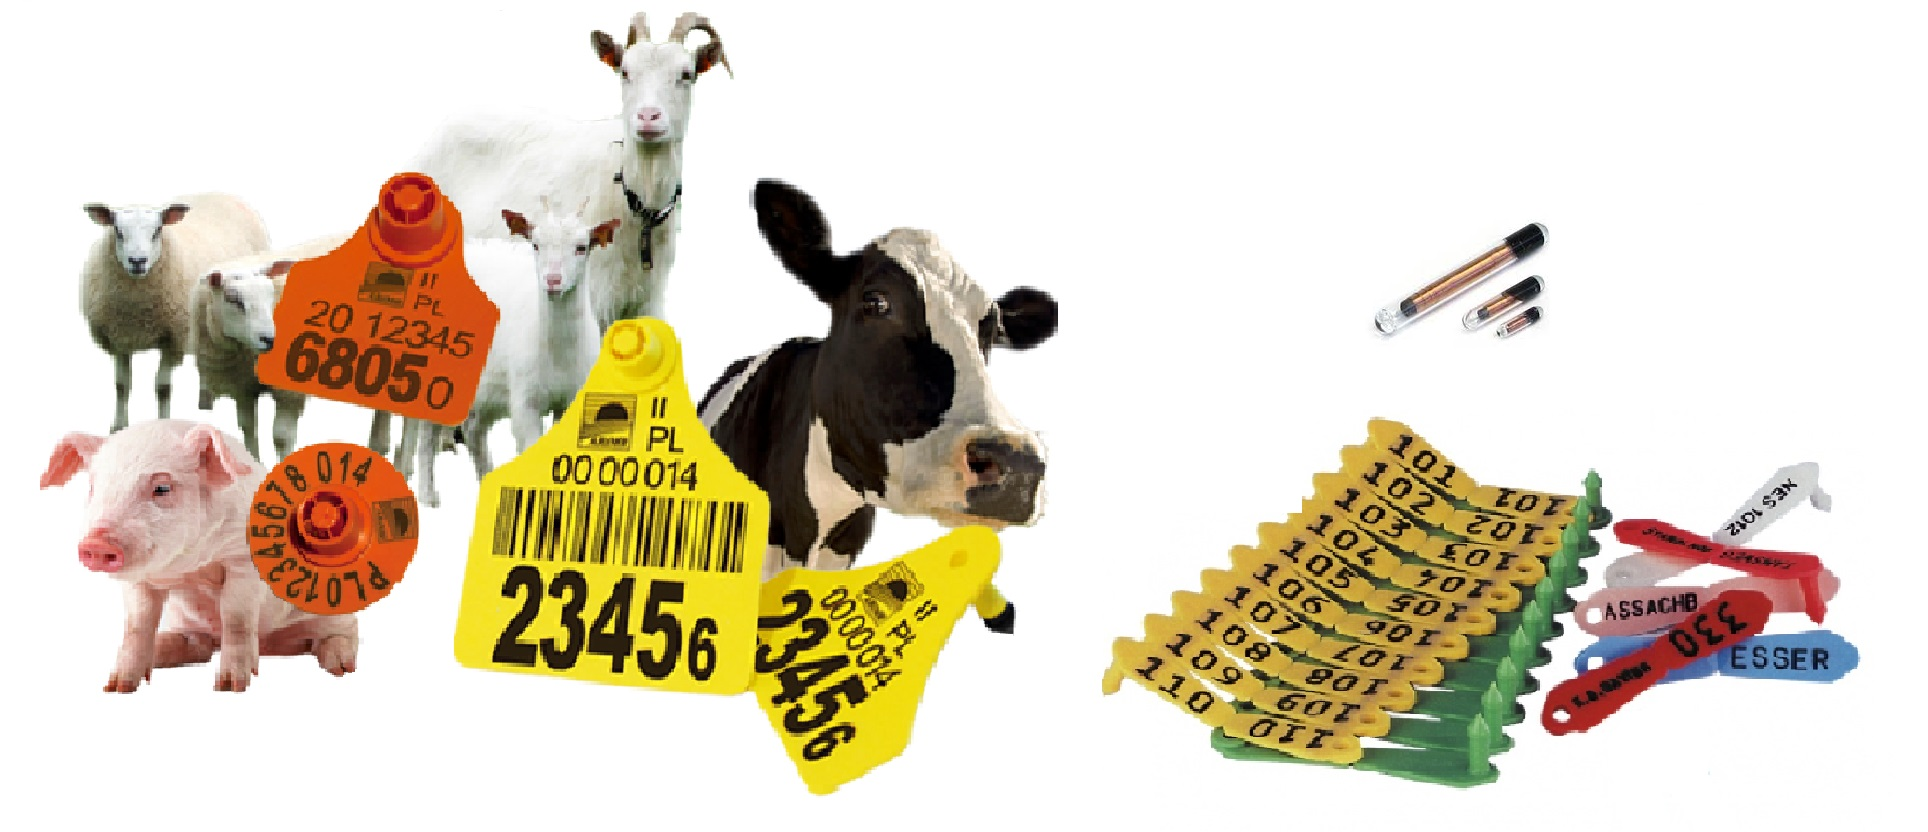
\includegraphics[width=14.34cm]{znakowanie_zwierzat.jpg}
	    \caption{Mikroczipy i kolczyki stosowane do znakowania zwierząt oraz kapsułki (biochipy) do wszczepiania pod skórę}
	\end{figure}
	
	Znaczniki LF zbudowane są z ferrytowego rdzenia, na którym nawinięte są zwoje cewki. Występują w formie plastikowych kart, krążków, biochipów, pastylek. Wadami systemu \emph{RFID-LF} są: mała szybkość transmisji danych (1-2 kb/sek), co znacznie ogranicza możliwą do zapisania / odczytania ilość danych, niewielki zasięg – około 0.5 metra, podatność na zakłócenia przez urządzenia elektryczne, co ogranicza zastosowanie w przemyśle, limit jednoczesnego odczytu nie więcej niż 20 transponderów – ogranicza to pojemność systemu i maksymalną liczbę odczytów jaką może obsłużyć jeden czytnik. 

	\item pasmo wysokich częstotliwości \emph{HF} (częstotliwości 6.78 MHz, 13.56 MHz, 27.125 MHz oraz 40.68 MHz). 
Transpondery \emph{HF} pracujące w zakresie 13.553 MHz – 13.657 MHz to zazwyczaj znaczniki pasywne. Identyfikatory pracujące na wysokich częstotliwościach wykazują się większą wrażliwością na obecność w swoim otoczeniu metali i mniejszym wpływem na zakłócenia elektromagnetyczne pochodzące od innych urządzeń niż znaczniki \emph{LF}. Pamięć znaczników \emph{HF} ma kilka razy większę pojemność, a szybkość komunikacji sięga 20 kbit/s. Cewka transpondera \emph{HF} zbudowana jest zazwyczaj z 3-8 zwojów, nadrukowana jest za pomocą przewodzącego lakieru na podłoże i zaprasowana w etykiecie. Znaczniki te produkowane są w postaci samoprzylepnych etykiet (ang.\emph{smart label}). Zaletami transponderów \emph{HF} są znacząco mniejsze koszty wykonania w porównaniu z identyfikatorami \emph{LF}, co spowodowane jest niewielką grubością identyfikatora, która osiąga nawet 0,1 mm. System RFID-HF daje możliwość odczytu do 50 znaczników jednocześnie (dzięki wprowadzeniu mechanizmów antykolizyjnych) co pozwala zastosować je do automatycznej identyfikacji produktów i obiektów. System wymaga zachowania odległości co najmniej 2-3 centymetrów pomiędzy transponderami. 
	
	Typowo zasięg działania systepu RFID pracującego w paśmie HF nie przekrasza 1,5 metra. Można uznać to za zaletę w przypadku systemu typu PayPass (płatności zbliżeniowe). Właściwość ta dodatkowo podnosi poziom bezpieczeństwa całego systemu, zmniejszając liczbę prób nieautoryzowanego dotępu.  

	\begin{figure}[h!]
	\centering
	    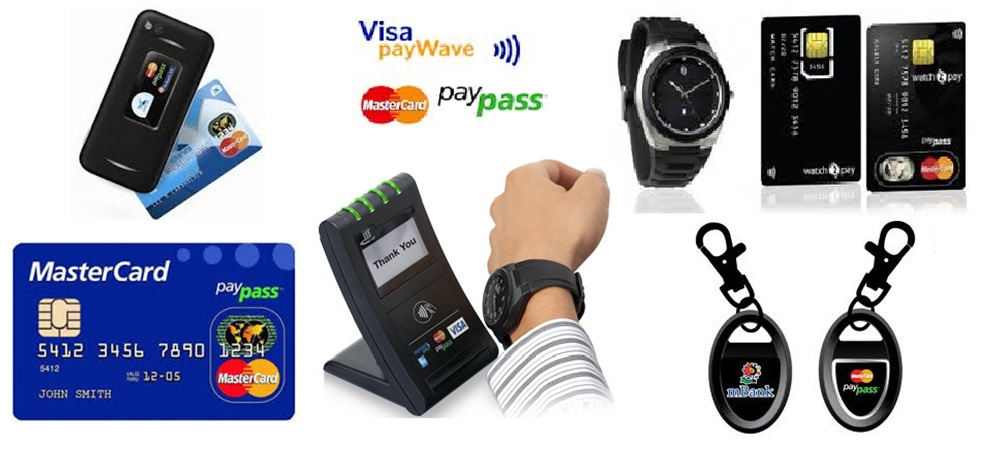
\includegraphics[width=16.56cm]{karty_platnicze.jpg}
	    \caption{Karty i breloki systemu PayPass}
	\end{figure}

	Systemy \emph{HF} są popularne ponieważ posiadają możliwość wielokrotnego zapisu danych, która jest niezbędna zarówno przy znakowaniu książek, dokumentów (paszportów, legitymacji studenckich, biletów komunikacji miejskiej, kart płatniczych) jak i bagażu na lotnisku, czy odzieży w pralni.

	\begin{figure}[h!]
	\centering
	    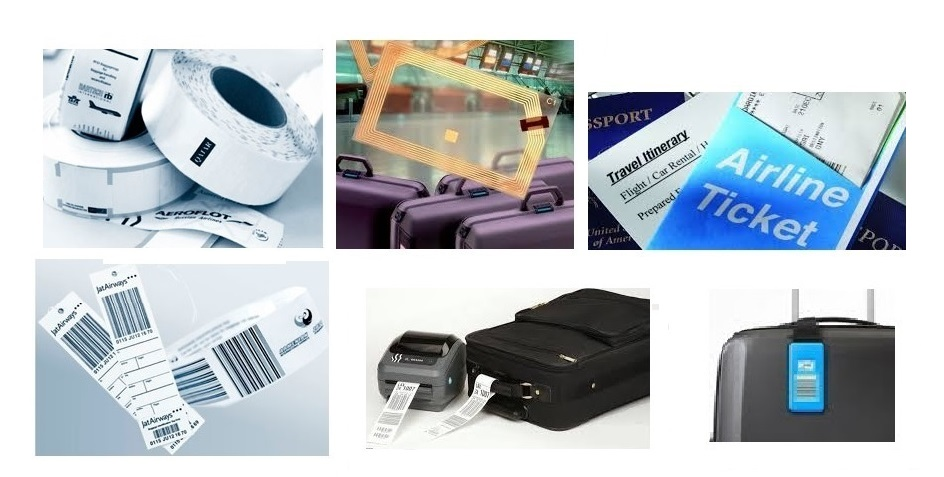
\includegraphics[width=15.51cm]{bagaz.jpg}
	    \caption{Znakowanie bagażu lotniczego}
	\end{figure}

	\begin{figure}[h!]
	\centering
	    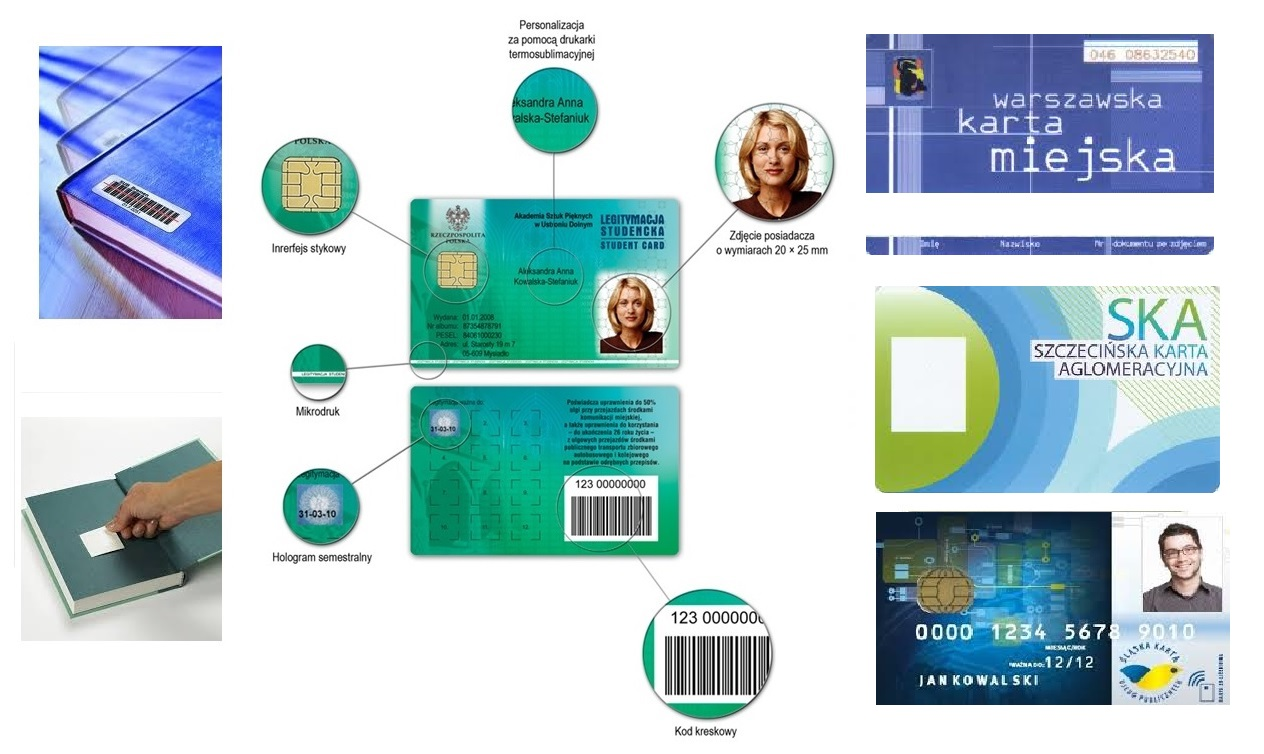
\includegraphics[width=16.82cm]{dokumenty.jpg}
	    \caption{Znakowanie książek, dokumentów, kart miejskich}
	\end{figure}
	
	 System znaczników pracujących na wysokich częstotliwościach znalazł zastosowanie w Europejskim Systemie Sterowania Pociągiem (ang. \emph{ETCS - European Train Control System}). System ten wyposażony w jest w urządzenie zwane Eurobalisą, które mocowane jest na torze pomiędzy szynami i może komunikować się z przejeżdżającymi nad nim pociągami.


	\item pasmo ultra wysokich częstotliwości \emph{UHF} (częstotliwości 433.92 MHz i 860-960 MHz).
Zakresy częstotliwości \emph{UHF} podzielono na kilka podzakresów np. Europa 860-868 MHz, Ameryka Północna 902-928 MHz, Japonia  950 MHz-956MHz. W związku z różnicami w częstotliwościach pracy urządzeń ustalono globalny standard ISO/IEC 18000-6 C. W celu objęcia globalnego łańcucha dostaw stworzono identyfikatory i czytniki, która mogą pracować na całym świecie. Znaczniki pasywne systemów \emph{RFID} pracujących w pasmie \emph{UHF} pozwalają na dużo większy zasięg niż znaczniki pasywne pozostałych pasm częstotliwości. Zaimplementowano lepsze protokoły antykolizyjne niż w systemach \emph{HF}. Wskutek tego zwiększyła się możliwość odczytu do 200 znacznikóa jednocześnie. Zasięg odczytu zawiera się w granicach od 3 do 6 metrów.Dodatkowo duża szybkość transmisji danych do 120 kbit/sek powoduje, że znajdują one zastosowanie w magazynach.

Podobnie jak znaczniki \emph{UHF} nie mogą być używane w pobliżu elementów metalowych, substancji płynnych i innych dobrych przewodników. 
Znaczniki \emph{UHF} ze względu na duży zasięg bardzo często stosowane są do śledzenia obiektów w logistyce. Wiele firm logistycznych, handlowych i spedycyjnych używa tylko i wyłącznie znaczników pasywnych \emph{UHF} ze względu na bardzo niski koszt produkcji, wynoszący kilkanaście groszy. 
Częstotliwość \emph{UHF} jest najbardziej rozpowszechnioną częstotliwością w logistyce i produkcji.

	\begin{figure}[h!]
	\centering
	    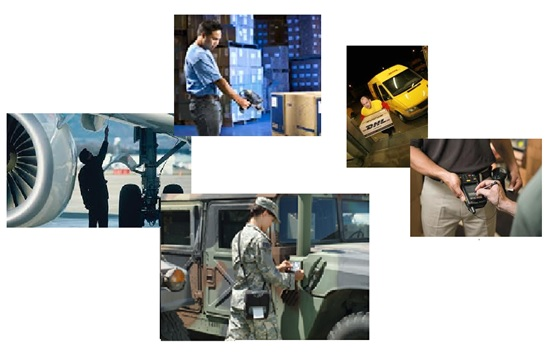
\includegraphics[width=14.37cm]{logistyka_transport_przemysl.jpg}
	    \caption{Przykłady zastosowań systemów RFID-UHF w sektorze logistyki, produkcji, transportu i handlu}
	\end{figure}

	\item pasmo mikrofalowe \emph{MW} (częstotliwości to 2.45 GHz, 5.8 GHZ i 24.125 GHz).
W paśmie \emph{MW} wykorzystuje się w większości znaczniki aktywne lub pasywno-aktywne. Są  mniejsze niż znaczniki pracujące na innych pasmach częstotliwości jednak droższe. Zasięg odczytu dochodzi do kilkuset metrów. Najistotniejszą zaletą tagów pracujących na częstotliwości mikrofalowej okazuje się wysoki transfer danych, który  umożliwia odczyt informacji z obiektów poruszających się z prędkością ponad 100 km/h, co nie jest możliwe w technologii tagów \emph{LF} i \emph{HF}. Pozwala to na wykorzystanie ich do identyfikacji środków transportu komunikacji miejskiej, samochodów poruszających się  na autostradzie (automatyczne naliczanie opłaty za przejazd autostradą), rejestracji przejeżdżających pociągów, czy statków.

	\begin{figure}[h!]
	\centering
	    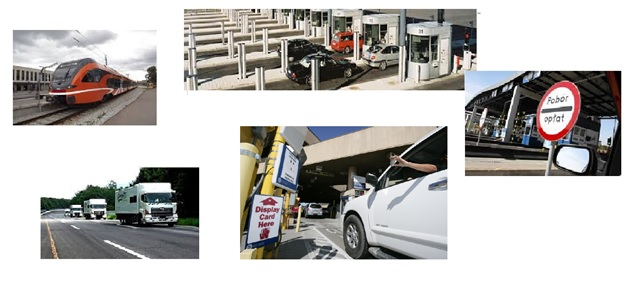
\includegraphics[width=16.61cm]{autostrady.jpg}
	    \caption{Naliczanie opłat za przejazd autostradą oraz identyfikacja środków komunikacji miejskiej}
	\end{figure}

	Znaczniki pracujące na częstotliwości 5.8 GHz montowane są w czujnikach przed drzwiami (w sklepach i marketach), w czujnikach ruchu jak również w systemach automatycznego spłukiwania toalet.
	Jedną z wad znaczników \emph{MW} jest możliwość wystąpienia zjawiska interferencji, które zakłóci  transmisję w środowisku o dużym zagęszczeniu znaczników jak również spowoduje zakłócenia w działaniu tych pracujących  w pobliżu substancji płynnych lub metali.

\end{itemize}

\newpage

\section{Główne obszary zastosowania systemów \emph{RFID}}

\noindent 
Technologia \emph{RFID} znalazła zastosowanie w niżej wymienionych sektorach gospodarki: 

\begin{itemize}\setlength{\itemsep}{0pt}
	\item logistyka, transport i magazynowanie – w przypadku konieczności szybkiej identyfikacji i śledzenia poszczególnych elementów łańcucha dostaw. Identyfikacja i rejestracja towarów w magazynie i na kolejnych etapach produkcji / dystrybucji.  Śledzenie przesyłek pocztowych / kurierskich, bagaży na lotnisku.  Znaczniki \emph{RFID} stopniowo wypierają etykiety logistyczne i kody kreskowe,

	\item płatności elektroniczne– systemy płatnicze PayPass, systemy kart rabatowych w hipermarketach i na stacjach benzynowych, 

	\item elektroniczne bilety, karty wstępu – komunikacja miejska, imprezy masowe/imprezy sportowe, opłaty za przejazd autostradami, systemy \emph{skipass},

	\item organizacja pracy – kontrola dostępu do wyznaczonych miejsc poprzez umieszczanie znaczników \emph{RFID} w identyfikatorach (np. kartach, breloczkach). Pozwalają one na identyfikację właściciela, monitoring czasu pracy oraz system kontroli dostępu (inteligentne budynki),

	\item znakowanie zbiorów, odzieży – archiwa, muzea i biblioteki w których na książkach coraz częściej zamiast kodów kreskowych znajdują się znaczniki RFID, które ułatwiają identyfikacje jak również zabezpieczają przed kradzieżą. Znakowanie odzieży w celu rozpoznawania i sortowania m.in. pralniach jak i w sklepach również w celu ochrony przed kradzieżą jak i fałszerstwem produktów markowych,
 	
 	\item dokumenty, papiery wartościowe– znaczniki w postaci samoprzylepnych etykiet. Śledzenie i zapisywanie historii obiegu oraz aktualnej lokalizacji ważnych dokumentów.  W paszportach stosowane w celu przechowywania danych osobowych oraz informacji na temat przekraczanych granic. Wymagane zabezpieczenie przed odczytem danych przez niepowołane osoby,
	
	\item przemysł – oznaczanie i  identyfikacja podzespołów, półproduktów oraz zapis poszczególnych stanów procesów produkcyjnych, co pozwala na ich automatyzację. Śledzenie obiektów na liniach produkcyjnych, rejestracja danych. Identyfikacja cystern, wagonów pojemników w procesie produkcji
	
	\item dane eksploatacyjne maszyn – identyfikacja tonerów do drukarek tak, aby drukarki nie podejmowały pracy w momencie przekroczenia dopuszczalnej liczby wydrukowanych stron na jednym tonerze lub w przypadku gdy toner nie pochodzi do konkretnego producenta, 
	
	\item rolnictwo, znakowanie zwierząt hodowlanych, zagrożonych gatunków – oznakowanie zwierząt za pomocą znaczników występujących w postaci charakterystycznych żółtych klipsów przymocowywanych do uszu bydła i trzody chlewnej. Pozwalają na identyfikację zwierząt a co za tym idzie odczytanie m.in. miejsca ich chowu,
	
	\item sport – rejestrowanie czasów oraz ilości okrążeń w zawodach sportowych. 
	
	\item transpondery na oponach samochodowych – zawierają najczęściej numer identyfikacyjny, datę produkcji oraz stopień zużycia opony.

\end{itemize}


\section{Wykorzystanie technologii \emph{RFID} w różnych sektorach gospodarki}

	\begin{figure}[h!]
	\centering
	    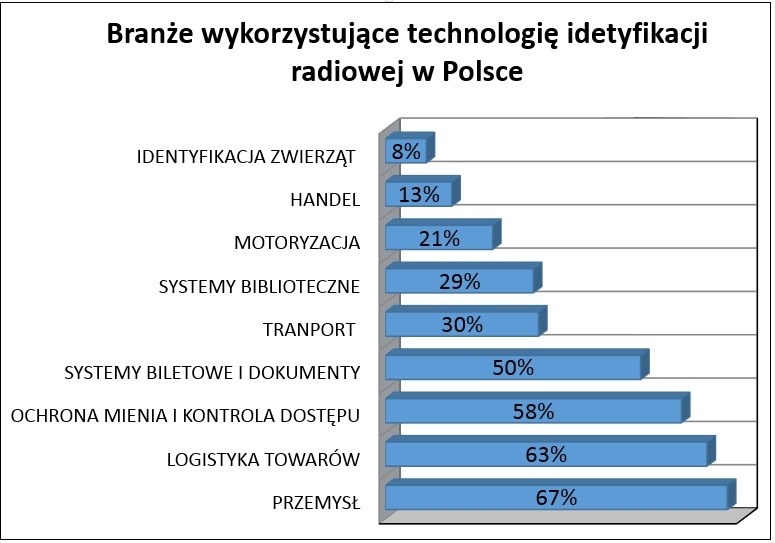
\includegraphics[width=16.2cm]{wykres_ver3.jpg}
	    \caption{Procentowy udział branż wykorzystujących technologię \emph{RFID}}
	\end{figure}


\section {Zalety i wady zastosowania systemu \emph{RFID}}

\noindent 
Zalety technologii \emph{RFID}:

\begin{itemize}\setlength{\itemsep}{0pt}
	\item nie jest wymagany optyczny kontakt zarówno przy zapisie jak i odczycie, czytnika z identyfikatorem, dzięki temu operację ta można zautomatyzować i zrealizować szybciej,
	
	\item możliwość odczytu wielu identyfikatorów równocześnie,
	
	\item duża pojemność pamięci, możliwość przechowywania większej ilości danych niż w przypadku kodów kreskowych

	\item możliwość aktualizacji / zmiany, wielokrotnego zapisywania i dopisywania danych  na etykiecie,

	\item identyfikatory mogą być wykorzystane wielokrotnie,

	\item duża prędkość transmisji danych,

	\item możliwość zapisywania danych w trakcie ruchu obiektu,

	\item duże bezpieczeństwo danych -istnieje możliwość zastosowana różnych metod ochrony danych zapisanych na znaczniku, zabezpieczenie dostępu do pamięci, zabezpieczenie dostępu hasłem,  

	\item miniaturyzacja znacznika - najmniejszy wyprodukowany na świecie znacznik przez firmę Hitachi posiada wymiary 0,05 x 0,05 mm

	\item możliwość pracy w trudnych warunkach przemysłowych w miejscach, gdzie występuje duże zapylenie, bardzo wysokie lub bardzo niskie ciśnienie, niska temperatura, agresywne środowisko chemiczne np. kopalnie, zakłady przemysłowe, chłodnie itp.

	\item możliwość integracji z istniejącymi systemami automatycznej identyfikacji (kody kreskowe),

	\item możliwość wykorzystania tych samych identyfikatorów w całym łańcuchu dostaw.

\end{itemize}

\noindent 
\newline Wady technologii \emph{RFID}:


\begin{itemize}\setlength{\itemsep}{0pt}

	\item brak jednolitego standardu dla protokołu RFID,
	
	\item możliwość zakłócenia przez odziaływanie elektromagnetyczne, wilgoć czy metale,
 	
 	\item większy koszt pojedynczego znacznika, w porównaniu z kodem paskowym, zwłaszcza w przypadku znaczników o większej funkcjonalności 

\end{itemize}





\chapter{Technologia anten konforemnych}

Układy antenowe o elastycznych, giętkich podłożach są trudne technologicznie do wykonania jednak mają szerokie zastosowanie praktyczne ze względu na możliwosć kształtowania powierzchni. 
W trakcie realizacji konforemne anteny i układy antenowe sprawiają wiele problemów konstrukcyjnych, gdyż nawet małe deformacje i odkształcenia mają duży wpływ na ich parametry polowe. 
Anteny konforemne dają możliwość uzyskania szerszego pokrycia kątowego płaszczyzny skanowania. Celem uzyskania poprawnych charakterystyk promieniowania należy w trakcie projektowania takich anten uwzględnić zmiany amplitud i faz sygnałów otrzymanych na poszczególnych elementach promieniujących, będących wynikiem chociażby odkształcenia ich struktury.    
Metody projektowania i konstruowania anten są na tyle skomplikowane, że cały proces łącznie z badaniami, aż do praktycznej realizacji przebiega z udziałem grupy sapecjalistów z różnych dziedzin (kompatybilności elektromagnetycznej, technologii materiałowych, systemów tekstronicznych, radioelektroniki, telekomunikacji, przetwarzania sygnałów i innych). Anteny o elastycznej strukturze przeznaczone są głownie do wykorzystania w pasmie powyżej 1 GHz.     

\section{Obszary wykorzystania i zastosowania anten konforemnych}

Możliwości zastosowania tego typu anten jest wiele. Dziedziny zastosowań wzajemnie się przenikają i uzupełniają, jednak można wyróżnić trzy najbardziej rozpowszechnione zastosowania, do których należą:

\begin{itemize}\setlength{\itemsep}{0pt}
	
	\item zastosowania medyczne - radary przenzaczone do mocowania na skórze: sportowców, ratowników medycznych, strażaków, żołnierzy. Czujniki służą do monitorowania aktywności (rytmu serca, oddechu) i stanu fizjologicznego człowieka (poziomu wydzielanego potu, stężenie tlenu i dwutlenku węgla we krwi, stanu odwodnienia, poziomu elektrolitów).Przekazywanie informacji o parametrach życiowych (np.temperaturze ciała). Wykrywanie zewnętrznych zagrożeń np. stężenie niebezpiecznych substancji chemicznych, gazów, oparów. Możliwość zaastosowana do wykrywania komórek nowotworowych,  

\begin{figure}[h!]
\centering
	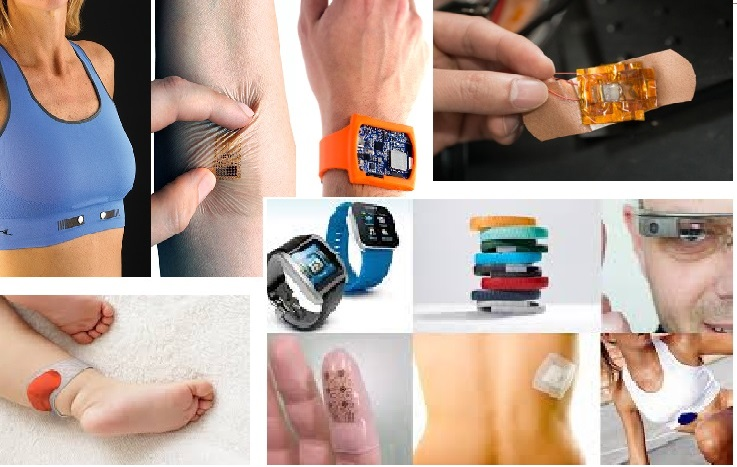
\includegraphics[width=14cm]{anteny_konforemne.jpg}
	\caption{Przykłady zastosowań anten konforemnych}
\end{figure}

	\item zastosowania militarne - system lokalnych sieci WBAN, wspieranie systemów rozpoznawania terenu UAVs (mobilny system łącznosci), określanie lokalizacji np. żołnierza, maskowanie aparatury do łączności.
	Zastapienie kilku urządzeń monitorujących systemem anten, a więc zmniejszenie wagi potrzebnego sprzętu. Zwiększenie niezawodności łączności (z ratownikami medycznymi, żołnierzami), a co za tym idzie poprawa mobilności służb,      

	\item zastosowanie to tworzenia krótkodystansowych systemów łączności bezprzewodowej - zastsowanie w sieciach: \emph{WPAN} (ang.\emph{Wireless Personal Area Network}), \emph{WBAN} (ang. \emph{Wireless Body Area Network}) oraz \emph{UWB} (ang. \emph{Ultra WideBand}). Współpraca czujników wszytych w ubranie (monitorowanie oznak życia organizmu). Integracja anten z elementami wyposażenia: kamizelką, rękawem, kołnierzem, hełmem (np. strażaka, żołnierza, policjanta) przy wykorzystaniu technologii Bluetooth, standardów GSM lub UMTS. Kominikacja anten z urzadzeniami działającymi w sieciach Wireless USB, Bluetooth, WLAN.  

\end{itemize}
	

\section{Częstotliwosci pracy dla anten konforemnych}
 
\noindent Pasma pracy:

\begin{itemize}\setlength{\itemsep}{0pt}
	
	\item UWB/WUSB: 3.1GHz - 10.6 GHz (FCC) - pasmo stosowane w systemach łączności krótkodystansowej, bazujące na przesyłaniu ultra-krótkich impulsów oraz charakteryzujące się niskim poborem mocy,

	\item ISM: 2.4 GHz - 2.4835 GHz - zakres używany przede wszystkim dla systemów łączności krótko i średniodystansowych takich jak Bluetooth, sieci WLAN / WBAN / WPAM,

	\item GPS: L1: 1575.42 MHz, L2: 1227.6 MHz, Galileo: 1176.45 MHz - częstotliwość pracy wykorzystywana do dla nawigacji satelitarnych GPS, Galileo i innych oraz do współpracy Galileo z innymi systemami takim jak GPS, Glonass, Loran-C, UMTS.

	\item ZigBee: 868 MHz, 915 MHz, 2.4 GHz - częstotliwości te znalazły zastosowanie w tworzeniu bezprzewodowych sieci sensorycznych.

	\item Zastosowania militarne: 50-300 MHz pasamo pracy przeznaczone dla radarów przenośnych oraz kamizelek z zintegrowanymi systemami łączności (antenami).

\end{itemize}

\section{Anteny tekstylne}

Tekstronika jest nową gałęzią nauki, zajmującą się projektowaniem i budową inteligentnej odzieży. Jest wynkiem połączenia kilku dziedzin nauki m.in. nauki o materiałach, włókiennictwa, elektroniki, radiokumunikacji, kompatybilności elektromagnetycznej jak również informatyki. Tekstronika stwarza możliwość wykorzystania różnych metod transmisji sygnałów w układach antenowych (patrz Rys. 2.2). W ramach niniejszej pracy skoncentrowano się na transmisji bezprzewodowej w paśmie nielicencjonowanym 2.4 GHz - 2,4835 GHz.  
Anteny do zastosowań tekstronicznych, czyli implementowane w odzieży, dzięki eleastycznej i giętkiej konstrukcji są łatwe do integracji z materiałami.


\begin{figure}[h!]
	\centering
	    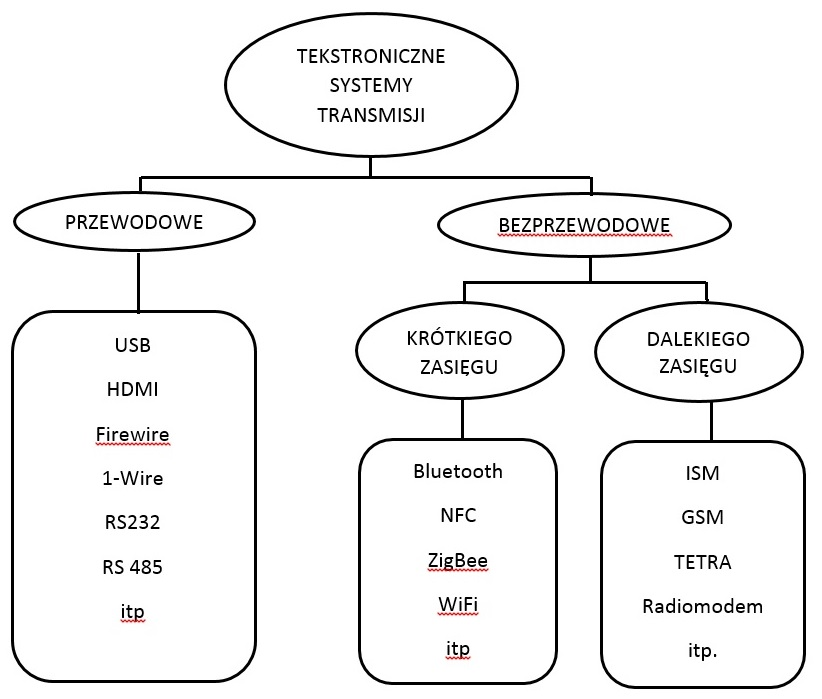
\includegraphics[width=15.5cm]{diagram.jpg}
	    \caption{Podział tekstronicznych systemów transmisji}
\end{figure}


 \chapter{Cel i zakres pracy}

Celem niniejszej pracy było zaprojektowanie i wykonanie anteny tekstylnej przewidzianej do pracy w paśmie \emph{ISM} (2.4 GHz). 
Praca nad projektem inżynierskim przebiegała w kilku etapach:

\begin{itemize}\setlength{\itemsep}{0pt}
	
	\item stworzenie modelu symulacyjnego badanej anteny,

	\item symulacje zaproponowanej struktury anteny,

	\item przeprowadzenie analizy numerycznej,

	\item wykonanie modelu i pomiar wybranych parametrów anteny.

\end{itemize}

Wszystkie symulacje numeryczne przeprowadzone zostały w srodowisku \emph{CST Microwave Studio}. Program umożliwia zaprojektowanie i przeprowadzenie dokładnych symulacji prototypu anteny. .................



\chapter {Projekt anteny}

\section{Wstęp}

\noindent Parametry anten istotne w procesie projektowania: 

\begin{itemize}\setlength{\itemsep}{0pt}

	\item pasmo pracy - czyli zakres częstotliwości, dla których projektowana antena spełnia założone wcześniej kryteria. Pasmo pracy anteny powinno być możliwie szerokie - dla anten RFID nie powinno jednak przekraczać 30 MHz,

	\item ipedancja wejściowa - jest to stosunek napięcia do natężenia prądu na zaciskach wejściowych anteny. Na impedancję wpływa obecność innych anten lub obiektów znajdujących się w pobliżu.
	Standardowa impedancja linii transmisyjnych wynosi 50\(\Omega\),

	\item zysk energetyczny - defionowany jako zysk kierunkowy zględem anteny wzorcowej (anteny izotropowej).
	Jest to stosunek gęstości mocy promieniowania w danym kierunku do średniej gęstości mocy wypromieniowanej przez antenę w pełnym kącie bryłowym. Podawany zazwyczaj dla kierunku, w którym promieniwanie anteny jest najsilniejsze, 

	\item charakterystyka promieniowania - pokazuje w jaki sposób antena promieniuje energię w różnych kierunkach. Obrazuje unormowany rozkład pola elektrycznego. Charakterystyka może być wyznaczona w dwóch płaszczyznach lub mieć postać trójwymiarową,

	\item polaryzacja anteny - określa ją polaryzacja wytwarzanej przez nią fali elektromagnetcznej 
	Wyróżniamy polaryzację liniową (pionową, poziomą, nachyloną pod kątem), eliptyczną lub kołową ( lewoskrętną, prawoskrętną),

	\item sprawność - to storunek mocy wypromieniowanej przez antenę do mocy dostarczonej do anteny,

	\item dopasowasowanie - linia transmisyjna jest dopasowana gdy impedancja wejściowa linii równa jest impedancji wejsciowej anteny. 

\end{itemize}

\newpage
\section{Struktura anteny}

Prototyp anteny tekstylnej RFID przesymulowano w środowisku \emph{CST Microwave Studio}. Inspiracją do stworzenia struktury wyjściowej był artykuł z 6th European Conference on Antennas and Propagation \cite{Artykul}. Strukturę bazową poddano modyfikacji celem dostosowania jej do założeń projektu. Optymalizacji parametrów symulacji, dokonano poprzez wybór opcji \emph{adaptive mesh refinement}, która ma na celu dostosowanie rozmiaru siatki, dzięki czemu otrzymane wyniki są dokładniejsze.


\begin{figure}[h!]
	\centering
	    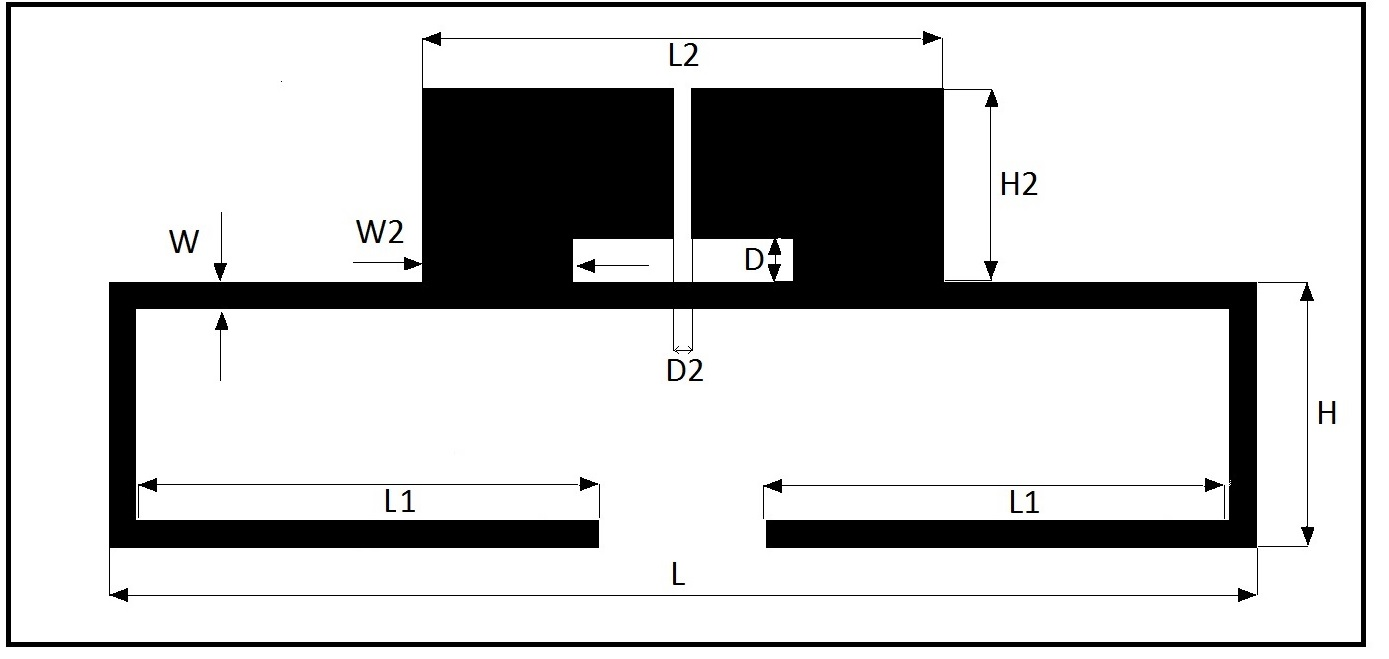
\includegraphics[width=15.5cm]{struktura.jpg}
	    \caption{Model struktury anteny}
\end{figure}


\begin{figure}[h!]
	\centering
	    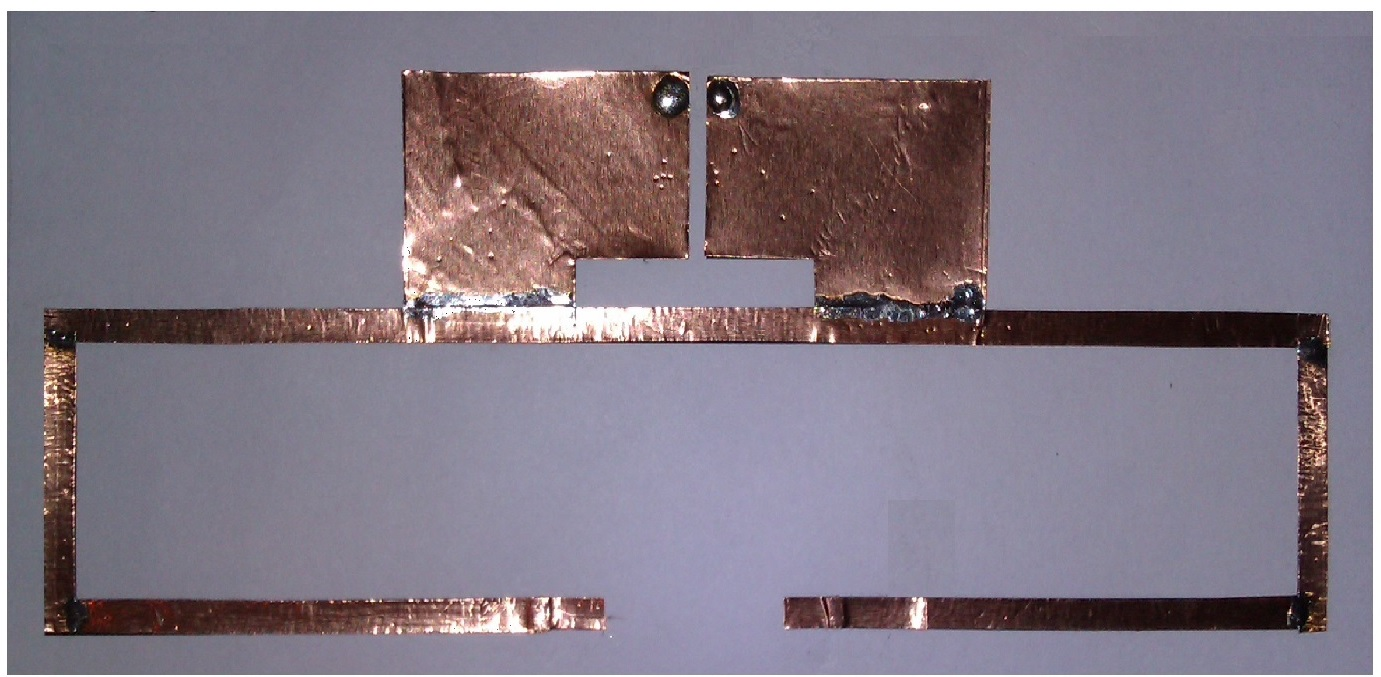
\includegraphics[width=15.5cm]{fizyczna_antena.jpg}
	    \caption{Prototyp anteny}
\end{figure}

\begin{table}[h]
\begin{center}
    \begin{tabular}{|c|c|}
    \hline
    ~                 & ~       \\
    PARAMETR          & WARTOŚĆ \\
    ~                 & ~       \\ \hline
    ~                 & ~       \\
    L                 & 130 mm  \\
    ~                 & ~       \\ \hline
    ~                 & ~       \\
    L1                & 55.5 mm \\
    ~                 & ~       \\ \hline
    ~                 & ~       \\
    L2                & 59 mm   \\
    ~                 & ~       \\ \hline
    ~                 & ~       \\
    H                 & 30 mm   \\
    ~                 & ~       \\ \hline
    ~                 & ~       \\
    H2                & 22 mm   \\
    ~                 & ~       \\ \hline
    ~                 & ~       \\
    D                 & 5 mm    \\
    ~                 & ~       \\ \hline
    ~                 & ~       \\
    D2                & 2 mm    \\
    ~                 & ~       \\ \hline
    ~                 & ~       \\
    W                 & 3 mm    \\
    ~                 & ~       \\ \hline
    ~                 & ~       \\
    W2                & 17 mm   \\
    ~                 & ~       \\ \hline
    ~                 & ~       \\
    DLUGOŚĆ PODŁOŻA   & 15.5 mm \\
    ~                 & ~       \\ \hline
    ~                 & ~       \\
    SZEROKOŚĆ PODŁOŻA & 7.5 mm  \\
    ~                 & ~       \\ \hline
    \end{tabular}
	\caption{Wymiary struktury anteny}
\end{center}
\end{table}



\begin{figure}[h!]
	\centering
	    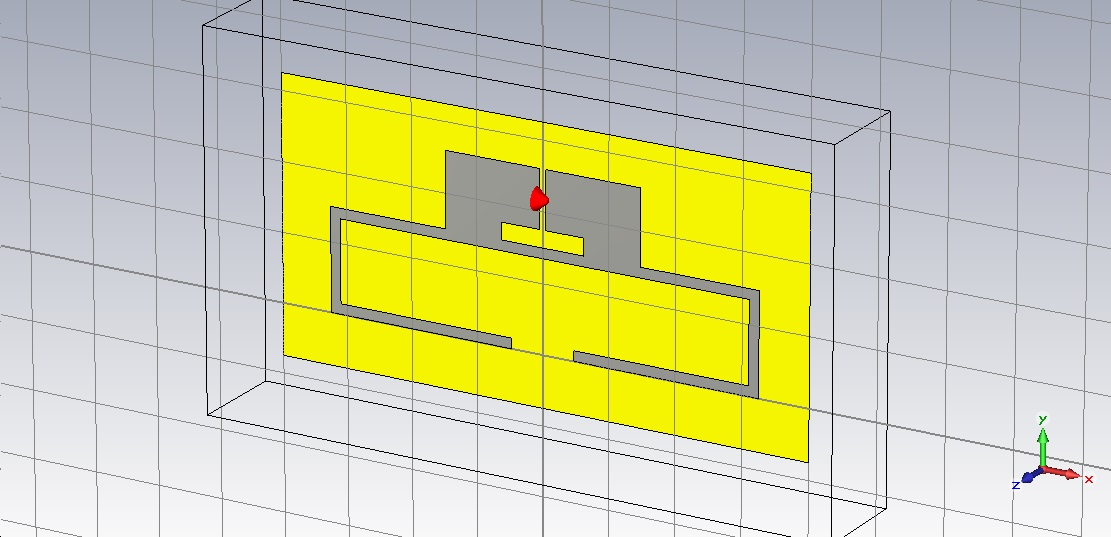
\includegraphics[width=15.5cm]{struktura_plaska.jpg}
	    \caption{Model struktury anteny z programu \emph{CST Microwave Studio}}
\end{figure}


Celem uzyskania w trakcie symulacji parametrów zbliżonych do założeń projektu przeprowadzono parametryzację struktury. Stopień dyskretyzacji został ustalony po 6 iteracjach. Rezultaty procesu doboru wymiarów anteny, można było obserwować na wykresach. Najlepsze wyniki posłużyły do ustalenia rozmiaru projektowanej anten, a pózniej wykonania prototypu. W rezultacie impedancja wejściowa symulowanej anteny wynosi 38 \(\Omega\). Schemat struktury po parametryzacji i prototyp pokazano na Rys.4.1 i Rys. 4.2. Wymiary zaprojektowanej anteny przestawiono w Tab. 4.1. 
\noindent 
\newline Wykonana antena ma strukturę dipola o polaryzacji poziomej z układem dopasowującym. 
Podłoże wykonano z papieru (aby struktura anteny była elastyczna i giętka, a co za tym idzie możliwy był jej pomiar na ramieniu cżłowieka).Przenikalność elektryczną podłoża przyjęto jak dla papieru $\epsilon_{r}$ = 2.31.

\section{Struktura anteny tekstylnej}

W programie \emph{CST Microwave Studio} zaprojektowano  model anteny tekstylnej naramiennej. Do celów symulacji dla modelu ramienia przyjęto $\frac{2}{3}\epsilon_{r}$ i $\frac{2}{3}\sigma$ dla mięśni czyli w tym wypadku $\epsilon_{r}$ = 35,193 i $\sigma$ = 1,14.

\begin{figure}[h!]
	\centering
	    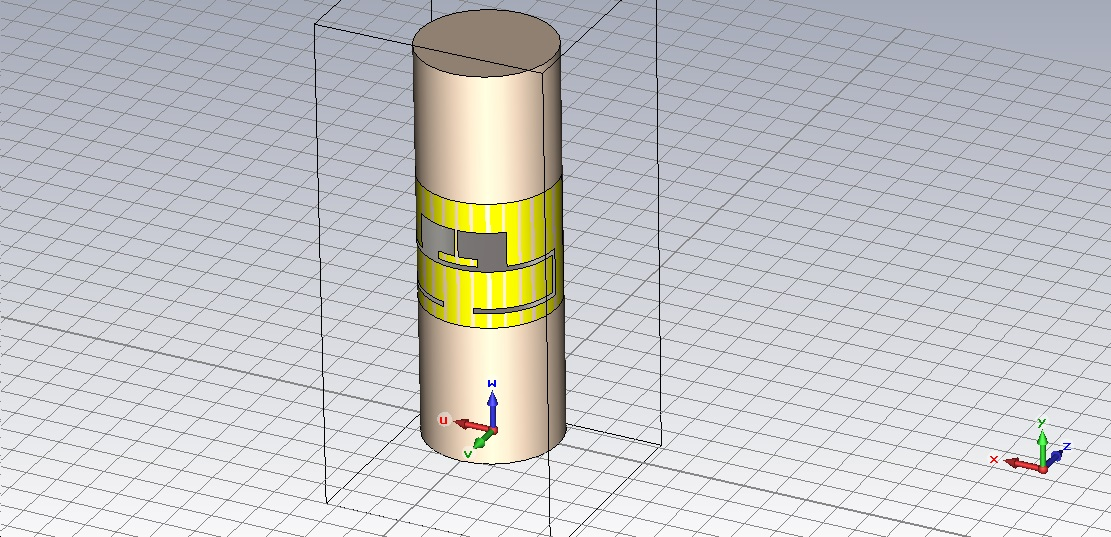
\includegraphics[width=15.5cm]{struktura_ramie.jpg}
	    \caption{Model struktury anteny tekstylnej naramiennej z programu \emph{CST Microwave Studio}}
\end{figure}


\chapter{Wyniki pomiarów}

\section{Pomiar i porównanie parametru $s_{11}$}

Pomiar parametru rozproszenia $s_{11}$ został przeprowadzony analizatorem widma firmy Agilent typu N5230A. Następnie otrzymane wyniki zostały porównane z wynikami uzyskanymi na podstawie symulacji w programie \emph{CST Microwave Studio}. Jak widać na Rys. 5.1 uzyskany przebieg symulacji różnił się od pomiarów przeprowadzonych na fizycznej antenie. W trakcie pomarów na kabel zasilający antenę zostały nałożone koraliki ferrytowe, aby zmniejszyć do minimum promieniowanie kabla i ewentualne zakłócenia z tym związane. 


\begin{figure}[h!]
\centering
	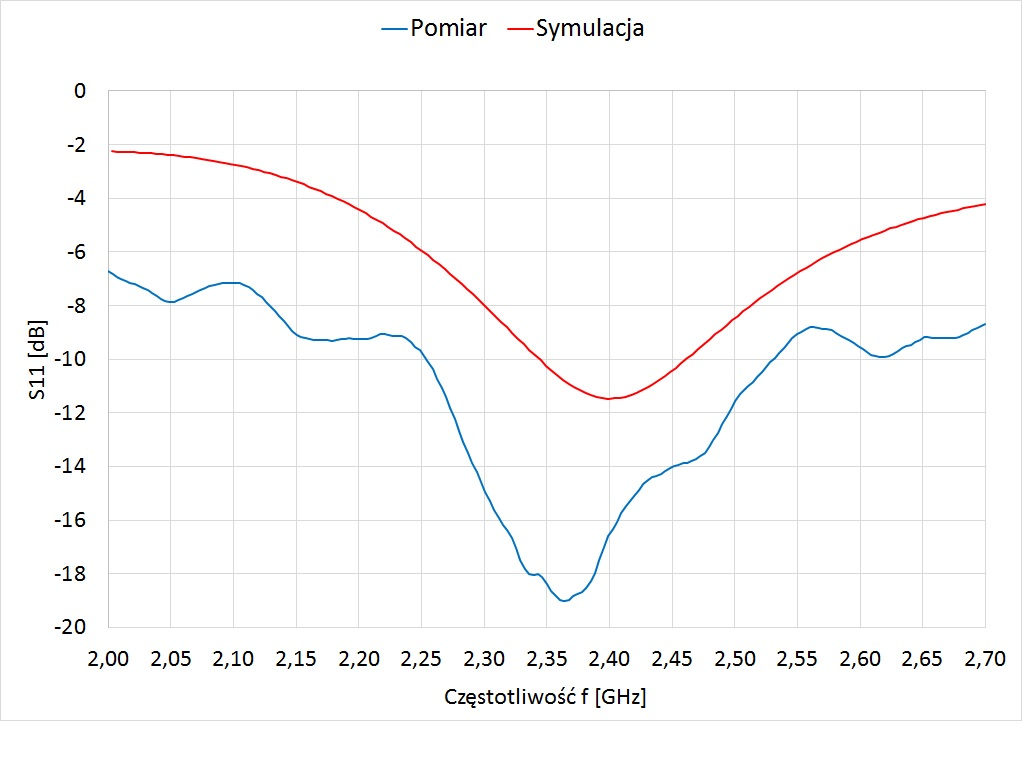
\includegraphics[width=16cm]{POM_Prz_Ko_SYM_Prz_Ko.jpg}
	\caption{Wykres zależności parametru $s_{11}$ od czestotliwości dla anteny przed korektą, porównany z wynikami symulacji}
\end{figure}


\newpage
Dla celów symulacji pryzjęto przenikalność elektryczną podłoża jak dla papieru $\epsilon_{r}$ = 2.31. Celem poprawy częstotliwości pracy wykonanej anteny konieczne okazały się modyfikacje struktury. Wprowadozne zmiany polegały na skróceniu odpowiednio długości anteny, aby mogła ona pracować na częstotliwośći rezonansowej. Długość \emph{L1} jednego ramienia skrócono o 7 mm a długość drugiego ramienia o 4 mm. Zauwążyć można, żę dla wykonanej anteny częstotliwość rezonansowa nieco spadła w porównaniu z symulacją. Jednak przeprowadzona modyfikacja długości ścieżek \emph{L1} przesuneła częstotliwość w oczekiwaną wartość \emph{F=2,3654 GHz}.   


\begin{figure}[h!]
\centering
	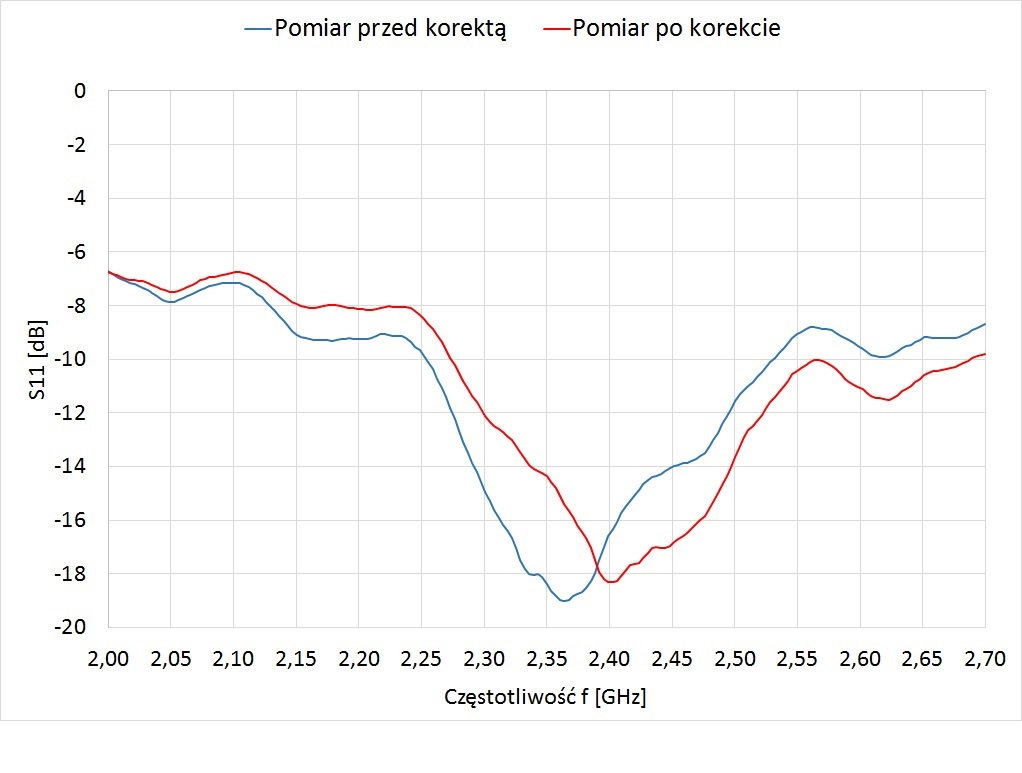
\includegraphics[width=16cm]{POM_Prz_Ko_POM_Po_Ko.jpg}
	\caption{Wykres zależności parametru $s_{11}$ od czestotliwości dla anteny przed korektą, porównany z wynikami anteny po korekcie}
\end{figure}


\noindent
\newline Umieszczenie anteny na ramieniu człowieka spowodowało przesunięcie częstotliwości rezonansowej w "góre", która wynosi dla tego przypadku \emph{F=2,6349 GHz}(patrz Rys. 5.3). Winika to z faktu, iż parametry anten silnie zależą od właściwości ośrodka stratnego.  
Tkanka ludzka jest dielektrycznym, dyspersyjnym ośrodkiem stratnym o skończonej konduktywności. Ponaddto fale o takiej samej częstotliwośći (w ośrodku dyspersyjnym), rozchodzą się różną prędkością. 


\begin{figure}[h!]
\centering
	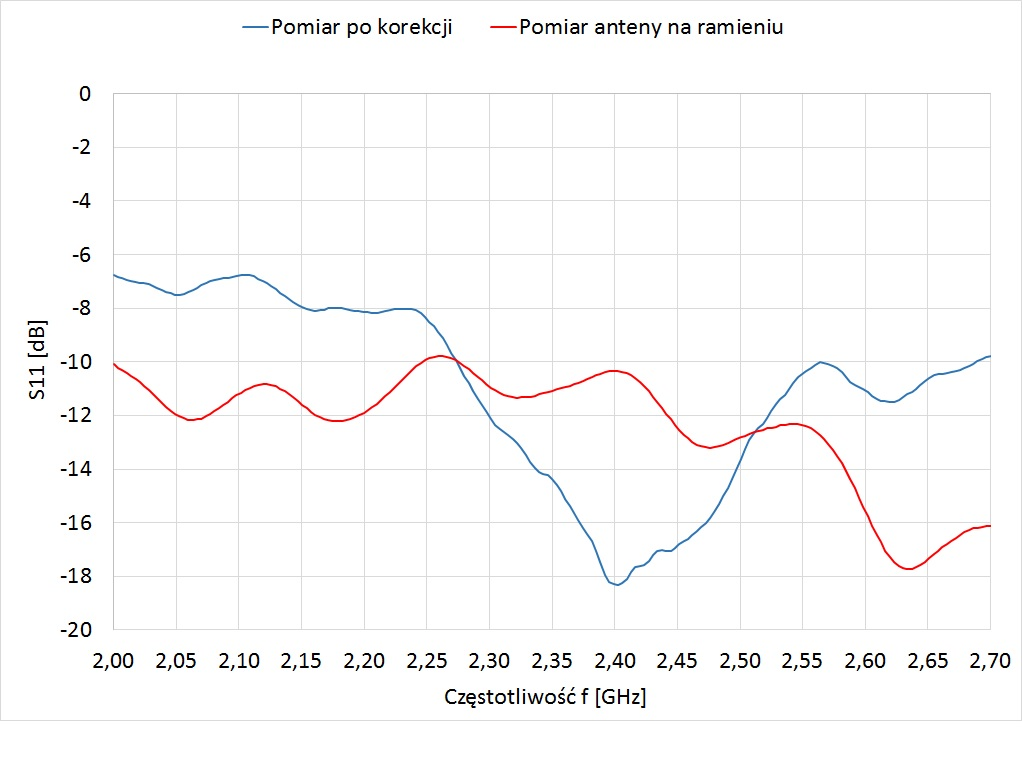
\includegraphics[width=16cm]{POM_Po_Ko_POM_Ram.jpg}
	\caption{Wykres zależności parametru $s_{11}$ od czestotliwości dla anteny po korekcji, porównany z pomiarami anteny umieszczonej na ramieniu}
\end{figure}



%Wpływ człowieka na charakterystykę promieniowania



%Obecność człowieka pogarsza charakterystykę promieniowania anteny. Zjawisko to spowodowane jest przewodzącymi właściwościami ciała człowieka, co powoduje tłumienie składowej elektrycznej pola. Na zakłócenia tego typu bardziej odporne są anteny pętlowe. Z tego powodu częściej znajdują one zastosowanie w urządzeniach przenośnych (np. pilotach zdalnego sterowania), na które mogłaby wpływać bezpośrednia bliskość człowieka.


\newpage 
\begin{table}[h]
\begin{center}
    \begin{tabular}{|c|c|c|}
    \hline
    ~                     & ~               & ~                         \\
     RODZAJ POLARYZACJI    & ANTENA WZORCOWA & ANTENA MIERZONA TEKSTYLNA \\
    ~                     & ~               & ~                         \\ \hline
    ~                     & ~               & ~                         \\
     POLARYZACJA POZIOMA  & -34.5 dBm       & -39,2 dBm                 \\
    ~                     & ~               & ~                         \\ \hline
    ~                     & ~               & ~                         \\
     POLARYZACJA PIONOWA  & -59.7 dBm       & -59.9 dBm                 \\
    ~                     & ~               & ~                         \\ \hline
    \end{tabular}
    \caption{Poziom mocy sygnału}
\end{center}
\end{table}




\begin{table}[h]
\begin{center}
    \begin{tabular}{|c|c|c|c|}
    \hline
    ~               & \multicolumn{3}{c|}{~}     \\
    ~               & \multicolumn{3}{c|}{ANTENA MIERZONA TEKSTYLNA } \\
    ~               & \multicolumn{3}{c|}{~}     \\ \hline
    ~               & \multicolumn{2}{c|}{~}     & ~                                  \\
    ANTENA WZORCOWA & \multicolumn{2}{c|}{BEZ OBECNOŚCI CZLOWIEKA} & W OBECNOŚCI CZLOWIEKA              \\
    ~               & \multicolumn{2}{c|}{~}     & ~                                  \\ \hline
    ~               & ~                          & ~                                  & ~                                  \\
    ~               & POŁOŻENIE ----             & POŁOŻENIE [     ]                  & POŁOŻENIE [    ]                   \\
    ~               & ~                          & ~                                  & ~                                  \\ \hline
    ~               & ~                          & ~                                  & ~                                  \\
    -10.24 dB       & -38.25 dB                  & -46.05 dB                          & -49.04 dB                          \\
    ~               & ~                          & ~                                  & ~                                  \\ \hline
    \end{tabular}
    \caption{Zysk energetyczny badanych anten}
\end{center}
\end{table}








\chapter{Podsumowanie}








 
%Tworzenie modelu symulacyjnego  Modelowanie      









%\begin{center}
%   \begin{tabular}{ | l | p{2.5cm} | p{2.5cm} | p{2.5cm} | p{2.5cm} |}
%    \hline
%        Smartphone OS & aaaa & bbbb & ccccc & dddd \\ \hline 
%      Android 2.2 & 299.94 & 509.32 & 164.76 & 537.95 \\ \hline
%       Android 2.3 & 133.50 & 154.76 & 57.65 & 215.13 \\ \hline
%        Android 4.0 & 97.05 & 103.44 & 31.80 & 179.36 \\ \hline
%        Android 4.1 & 75.60 & 85.57 & 21.60 & 132.03 \\ \hline
%       Android 4.2 & 55.28 & 83.76 & 23.28 & 121.51 \\ \hline
%       iPhone iOS5 & 21.61 & 132.90 & 8.64 & 177.69 \\ \hline
%        iPhone iOS6 & 15.71 & 73.86 & 7.27 & 109.32 \\ \hline
%    \hline
%    \end{tabular}
%\end{center}

%W poniżsyzm rozdziale 









	
%
%\chapter{Cel i zakres pracy} \label{sec:Cel i zakres pracy}
Celem pracy jest stworzenie aplikacji
mobilnej w j�zyku Java 2 Micro Edition prezentuj�cej mo�liwo�ci
wykorzystania standardu Bluetooth implementowanej w telefonach
kom�rkowych. Zakres pracy obejmuje r�wnie� opis wykorzystania
platformy Java w programowaniu mobilnym Ze szczeg�lnym
uwzgl�dnieniem klas \textbf{MediaAPI} umo�liwiaj�cej nagrywanie oraz
odtwarzanie d�wi�ku oraz \textbf{BluetoothAPI} b�d�cej implementacj�
wi�kszo�ci znanych serwis�w Bluetooth.

%
%\chapter{Bluetooth}
\label{sec:Bluetooth}
%
\section{Wstêp}
\label{sec:Wstep}
%
 Technologia Bluetooth jest standardem umo¿liwiaj¹cym bezprzewodow¹ komunikacjê
pomiêdzy ró¿nymi urz¹dzeniami elektronicznymi, takimi jak
klawiatura, komputer, laptop, palmtop, telefon komórkowy czy
urz¹dzenia audio. Interfejs Bluetooth pracuje w nielicencjonowanym
paœmie ISM (Industrial Scientific Medicine). W wiêkszoœci krajów
jest to zakres 2400 - 2483,5 MHz (wyj¹tkiem jest np. Francja i
Hiszpania, gdzie pasmo to ma zakres 2446,5 - 2483,5 MHz). Okreœlone
pasmo jest podzielone na 79 (Francja, Hiszpania: 23) kana³ów o
szerokoœci 1 MHz, które s¹ wykorzystywane w technice frequency
hopping. Polega ona na okresowej zmianie kana³u transmisyjnego w
celu unikniêcia zak³óceñ. W standardzie zmiana kana³u nastêpuje 1600
razy na sekundê , a urz¹dzenia maj¹ do wyboru 5 ró¿nych sekwencji
zmiany kana³ów tzw. hopping sequence, zgodnie z którymi dokonywane
s¹ zmiany czêstotliwoœci. Frequency hopping pozwala zmniejszyæ
zak³ócenia transmisji wyp³ywaj¹ce z pracy takich urz¹dzeñ jak
kuchenki mikrofalowe czy modu³y 802.11, pracuj¹ce w tym samym
zakresie czêstotliwoœci. Urz¹dzenia Bluetooth pozwalaj¹ na pracê w
zakresie mocy od 1 do 100 mW, co umo¿liwia transmisjê na odleg³oœci
od 10 do 100 m. Wiêkszoœæ urz¹dzeñ Bluetooth ogranicza jednak pobór
mocy do minimum i pozwala na pracê w odleg³oœciach do 10 m,
zmniejsza to tak¿e koszty produkcji uk³adu, gdy¿ nie musi on byæ
wyposa¿ony w modu³ kontroli mocy.

Zasiêg Bluetooth zale¿y od klasy mocy:

\begin{itemize}
    \item klasa 1 (100 mW) ma najwiêkszy zasiêg, do 100 m,
    \item klasa 2 (2,5 mW) jest najpowszechniejsza w u¿yciu, zasiêg do 10 m
    \item klasa 3 (1 mW) rzadko u¿ywana, zasiêg do 1 m.
\end{itemize}

 Transfer maksymalny okreœla edycja protoko³u
\begin{itemize}
    \item Bluetooth 1.0 - 721 kb/s
    \item Bluetooth 1.1 - 721 kb/s
    \item Bluetooth 1.2 - 721 kb/s
    \item Bluetooth 2.0 - transfer maksymalny przesy³ania danych na poziomie 2.1~Mb/s, Enhanced Data Rate - transfer do 3.0 Mb/s
\end{itemize}

Protokó³ Bluetooth nie jest jednak doskona³y. Zawiera w sobie luki,
które umo¿liwiaj¹ dostêp  z zewn¹trz do przesy³anych danych. Pakiety
Bluetooth mo¿na stosunkowo ³atwo przechwyciæ przy pomocy
specjalnych programów tzw. snifferów. Ponadto niektóre urz¹dzenia
wyposa¿one w Bluetooth, g³ównie ze wzglêdu na prostotê obs³ugi,
umo¿liwiaj¹ nawi¹zanie z nimi po³¹czenia bez jakiejkolwiek wiedzy
ich w³aœciciela. Istnieje jednak mo¿liwoœæ u¿ytkowania protoko³u
Bluetooth w taki sposób, ¿e ewentualne przechwycenie danych nie
stanowi ¿adnego zagro¿enia dla przesy³anych danych. Wystarczy
opakowaæ wysy³ane dane u¿ywaj¹c odpowiednich technik w warstwie
aplikacji. Wówczas pods³uchane dane po stronie ,,sniffera'' to
zaledwie ciąg bezu¿ytecznych bajtów.
%
\subsection{Topologia}
\label{sec:Mozliwosci} Komunikacja w technologii Bluetooth odbywa
siê na zasadzie master-slave. Po nawi¹zaniu po³¹czenia jedno z
urz¹dzeñ (inicjator po³¹czenia) staje siê masterem, drugie slavem
(przy czym urz¹dzenia Bluetooth s¹ pod tym wzglêdem nierozró¿nialne,
ka¿de mo¿e pe³niæ obie funkcje). Standard definiuje pojêcie piconetu
tj. sieci sk³adaj¹cej siê z jednego mastera i od jednego do siedmiu
aktywnych slave'ów, przy czym komunikacja zawsze odbywa siê poprzez
mastera. Nie ma wiêc mo¿liwoœci bezpoœredniej komunikacji pomiêdzy
slave'ami w ramach piconetu. Wiele piconetów tworzy poprzez
wspó³dzielenie wêz³ów wiêksz¹ sieæ tzw. scatternet. jak pokazano na
rysunku poni¿ej wêze³ po³¹czony z wiêcej ni¿ jednym piconetem mo¿e
byæ slavem we wszystkich z nich, lub masterem w jednym piconecie i
slave'm we wszystkich pozosta³ych.

\begin{figure}[b]
\centering
    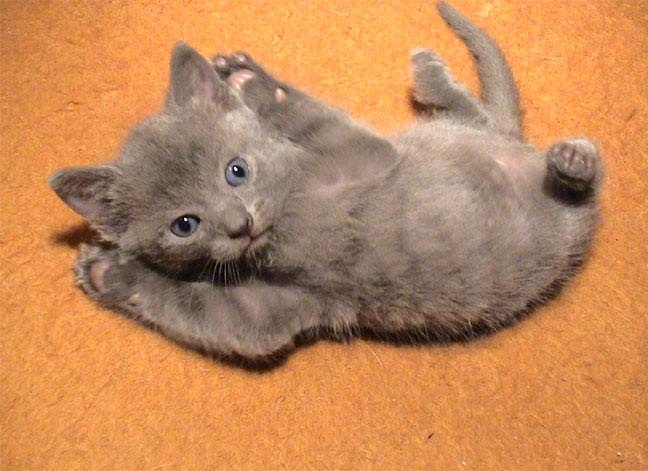
\includegraphics[width=50mm]{kot_d.jpg}
     \caption{Ka¿dy rysunek musi mieæ swój podpis!!}\label{F_cube}
\end{figure}


W zwi¹zku z tym, ¿e sieci Bluetooth tworzone s¹ ad-hoc a technologia
przeznaczona jest g³ównie dla urz¹dzeñ o charakterze przenoœnym
(mobilnym), elementy pico-sieci mog¹ czêsto ,,wychodziæ'' z zasiêgu
innych urz¹dzeñ lub siê w nim niespodziewanie ,,pojawiaæ''. Topologia
sieci i urz¹dzenia, które j¹ tworz¹, ulegaj¹ wiêc ci¹g³ym zmianom.
Protokó³ Bluetooth musi zawieraæ zatem kontroler  który ³¹czy
wykorzystuj¹c informacje wysy³ane przez ka¿de urz¹dzenie Bluetooth w
zasiêgu, zarz¹dza procesami wykrywania i kojarzenia urz¹dzeñ.
%
\section{Stos protoko³ów}\label{sec:stos}
Protokó³ Bluetooth jest wykorzystywany w urz¹dzeniach które mog¹ siê
ró¿nic technologicznie w zale¿noœci od zastosowania lub producenta.
Stos protoko³ów Bluetooth nie odpowiada ¿adnemu znanemu modelowi
(OSI, TCP/IP, 802) ale w przeciwieñstwie do wiêkszoœci protoko³ów
sieciowych, które okreœlaj¹ tylko kana³y pomiêdzy komunikuj¹cymi
siê jednostkami, stos protoko³ów Bluetooth w wersji 1.1 okreœla 13
specjalnych aplikacji, zwanych profilami systemu Bluetooth, w
których system mo¿e byæ u¿ywany.
%
\subsection{Warstwa Fizyczna}
\label{sec:Warstwa Fizyczna}

Warstwê fizyczn¹ Bluetooth stanowi interfejs radiowy o stosunkowo
niewielkim poborze mocy, dzia³aj¹cy na w zale¿noœci od klasy w
zasiêgu 1 - 100m. Warstwa radiowa Bluetooth operuje w paœmie ISM
2,4 GHz. Pasmo to jest podzielone na 79 kana³ów, po 1MHz ka¿dy.
System wykorzystuje modulacje FSK (Frequency Shift Keying) dziêki
której uzyskujemy prêdkoœci transmisji do 1 Mbit/s. Skakanie po
czêstotliwoœci odbywa siê z czêstoœci¹ 1600 skoków na sekundê.
Sekwencjê skoków dyktowane s¹ przez wêze³ master.
%
\subsection{Warstwa Baseband}
\label{sec:Warstwa Baseband} Warstwa baseband jest zbli¿ona do
podwarstwy MAC modelu OSI. Upakowuje ona luŸne bity w ramki. Master
w ka¿dej pikosieci definiuje sloty czasowe o d³ugoœci $625 \mu s$.
Transmisja mastera zaczyna siê od slotów parzystych natomiast
transmisja slave od slotów nieparzystych (multipleksacja w
dziedzinie czasu dziedzinie czasu - TDM). Ramki mog¹ mieæ d³ugoœæ
jednego, trzech lub piêciu slotów czasowych. Skakanie czêstotliwoœci
pozwala ustawiæ czas $250 - 260 \mu s$ na skok, aby umo¿liwiæ
stabilizacjê uk³adów radiowych. Ka¿da ramka jest transmitowana
przez kana³ logiczny, nazywany z angielskiego ,,link'', pomiêdzy
masterem i urz¹dzeniem slave. Istniej¹ dwa rodzaje kana³ów
logicznych. Pierwszy nazywa siê ACL (Asynchronous Connection-Less),
u¿ywany w po³¹czeniu z komutacj¹ pakietów, gdzie dane s¹ dostêpne w
nieregularnych odstêpach czasu. Dane te pochodz¹ od warstwy L2CAP po
stronie nadawczej i s¹ dostarczane do warstwy L2CAP po stronie
odbiorczej. W tej wersji kana³u logicznego nie ma ¿adnych gwarancji,
ze ramka dotrze do celu. Ramki mog¹ zostaæ utracone i wymagaæ
retransmisji. Urz¹dzenie slave mo¿e mieæ tylko jeden kana³ typu ACL
z urz¹dzeniem master. Drugi typ kana³u logicznego to SCO
(Synchronous Connection Oriented) i jest u¿ywany do transmisji w
czasie rzeczywistym, np. rozmowy telefonicznej z u¿yciem zestawu
s³uchawkowego. Ramki transmitowane w tego typu kanale, nie mog¹ byæ
retransmitowane. Zamiast tego mo¿na stosowaæ korektê b³êdów, aby
zapewniæ mo¿liwie wysok¹ niezawodnoœæ. Urz¹dzenie slave mo¿e
korzystaæ z maksymalnie trzech kana³ów typu SCO w kierunku mastera.
Ka¿de  SCO mo¿e transmitowaæ jeden kana³ telefoniczny (PCM,
64kbit/s).
%
\subsection{Protokó³ Voice}
\label{sec:Protokol Voice}

Protokó³ Bluetooth umo¿liwia przesy³anie sygna³ów wymagaj¹cych
transmisji synchronicznej, takich jak sygna³ mowy, a tak¿e sygna³ów,
które wymagaj¹ wiêkszych prêdkoœci transmisji, ale mog¹ byæ
przesy³ane asynchronicznie, czyli transmisji danych. Zdefiniowane s¹
dwa typy ³¹cz:
\begin{itemize}
\item  ³¹cza synchroniczne (SCO, Synchronous Connection Oriented),
\item  ³¹cza asynchroniczne (ACL, Asynchronous Connectionless).
\end{itemize}
Dostêpne s¹ pakiety ACL dwóch typów: DM (Data Medium) i DH (Data
High). Pakiety DH zawieraj¹ mniej informacji zwi¹zanych z korekcj¹
b³êdów, dziêki czemu umo¿liwiaj¹ wiêksz¹ prêdkoœæ transmisji.
Najszybsza transmisje umo¿liwiaj¹ pakiety DH5, które zajmuj¹ piêæ
szczelin czasowych. Pakiet taki mo¿e przenieœæ 339 bajtów (2712
bitów) danych, a wiec, aby przes³aæ 2712 bitów informacji, trzeba
przes³aæ 2854 bitów). W odpowiedzi na pakiet DH5, który zajmuje 5
szczelin, musi zostaæ przes³any pakiet o d³ugoœci co najmniej jednej
szczeliny. Daje to maksymalna przepustowoœæ w jednym kierunku równa
723,2 kb/s. W kierunku zwrotnym pakiety o d³ugoœci jednej szczeliny
przenios¹ 57,6 kb/s. Jeœli pakiety DH5 bêd¹ przesy³ane w obu
kierunkach, uzyskana przepustowoœæ w jednym kierunku bêdzie wynosi³a
433,9 kb/s. Ze wzglêdu na to, ze wy¿sze warstwy protoko³u Bluetooth
wymagaj¹ przesy³ania danych steruj¹cych, maksymalna przepustowoœæ na
poziomie aplikacji wynosi oko³o 650 kb/s. Koszty ponoszone na
kodowanie danych i skoki czêstotliwoœci s¹ niezbêdne, aby utworzone
³¹cze by³o niezawodne, poniewa¿ wykorzystywane pasmo ISM jest
wspó³u¿ytkowane przez wiele ró¿nego rodzaju urz¹dzeñ. Ograniczenia
s¹ tak¿e wymuszane przez lokalne przepisy, które ograniczaj¹ moc
promieniowana w jednostce czasu w pasmie ISM. Dziêki skokom
czêstotliwoœci transmisja jest rozpraszana w czêstotliwoœci i w
czasie. £¹cza SCO dzia³aj¹ z przepustowoœci¹ 64 kb/s. W jednym
czasie mo¿na korzystaæ z trzech ³¹czy g³osowych. Mo¿na tak¿e mieszaæ
w jednym ³¹czu dane g³osowe przesy³ane synchronicznie i dane
przesy³ane asynchronicznie. £¹cza SCO stanowi¹ symetryczne ³¹cza
miêdzy urz¹dzeniem nadrzêdnym i podrzêdnym o zarezerwowanej
przepustowoœci i zapewniaj¹ regularn¹, w okreœlonych odstêpach
czasu, wymianê danych w zarezerwowanych szczelinach czasowych. S¹ to
wiec ³¹cza umo¿liwiaj¹ce przekazywanie danych, dla których istotny
jest czas, a wiec na przyk³ad sygna³ów audio. Urz¹dzenie nadrzêdne
mo¿e obs³ugiwaæ do trzech ³¹czy z tym samym lub ró¿nymi urz¹dzeniami
podrzêdnymi, a urz¹dzenie podrzêdne mo¿e obs³ugiwaæ do trzech ³¹czy
z urz¹dzeniem nadrzêdnym. Pakiety SCO nie s¹ nigdy retransmitowane.
Protokó³ ten nie jest umieszczony w zestawie klas J2ME i nie mo¿e
byæ wykorzystany w aplikacjach mobilnych.

%
\subsection{HCI}
\label{sec:Warstwa HCI}

\textbf{Host Controller Transport} pozwala na transparentn¹ wymianê
informacji takich jak komendy HCI, dane ACL i SCO, dostarczenie
komend kontroluj¹cych pracê warstwy baseband i Link Manager. G³ównym
zadaniem HCI jest dostarczenie metod umo¿liwiaj¹cych korzystanie z
zasobów warstwy baseband protoko³u Bluetooth.

\subsection{LMP}
\label{sec:Warstwa LMP} \textbf{Link Manager Protocol} ustala
parametry ³¹cza, umo¿liwia nas³uchiwanie i wykrywanie urz¹dzeñ w
pobli¿u. LMP sk³ada siê z kilku PDU (protocol Data Units) które s¹ wysy³ane z
jednego urz¹dzenia do innego znajduj¹cego siê w zasiêgu w procesie
nawi¹zywania po³¹czenia. PDU s¹ wysy³ane jako single-slot z
jednobajtowym nag³ówkiem.
%
\subsection{Warstwa L2CAP}
\label{sec:Warstwa L2CAP}

Logical Link Control and Adaptation Layer Protocol jest warstw¹
maj¹c¹ za zadanie transmisjê danych do warstw wy¿szych zarówno w
sposób zorientowany po³¹czeniowo jak np. port szeregowy RFCOMM, jak
równie¿ bez po³¹czeniowo. Warstwa ta zawiera równie¿ zestaw metod do
multipleksowania i segmentacji danych oraz operacji odwrotnych
potrzebnych do przesy³ania danych pomiêdzy warstw¹ baseband a
warstwami wy¿szymi.

 Warstwa L2CAP spe³nia trzy g³ówne funkcje:
\begin{itemize}
  \item przyjmuje pakiety o maksymalnym rozmiarze do 64 KB od wy¿szych warstw i dzieli je na ramki w celu transmisji.
   Na koñcu ramki s¹ ponownie sk³adane w ca³oœæ.
  \item zajmuje siê multipleksacj¹ i demultipleksacj¹ z³o¿onych pakietów. Gdy pakiet jest sk³adany w ca³oœæ, warstwa L2CAP okreœla, któremu protoko³owi warstwy wy¿szej go przekazaæ, np. do RFcomm lub telephony.
  \item zajmuje siê wymaganiami na jakoœæ us³ugi, zarówno podczas zestawiania po³¹czenia oraz podczas realizacji us³ugi.
\end{itemize}

\emph{Segmentacja}

W porównaniu do innych mediów fizycznych, pakiety danych
zdefiniowane przez warstwê baseband maj¹ ograniczony rozmiar.
Wysy³anie maksymalnej iloœci danych zdefiniowane jest przez MTU
(maximum transmission unit) i przy maksymalnym wykorzystaniu pasma
wynosi 341 bajtów na pakiet DH5. Wy¿sze warstwy z regu³y
przystosowane s¹ do obs³ugi znacznie wiêkszych "porcji" danych,
dlatego du¿e pakiety L2CAP musz¹ byæ podzielone na segmenty tak aby
ich przesy³ drog¹ radiow¹ by³ mo¿liwy przy okreœlonych parametrach
³¹cza. W podobny sposób segmenty odbierane z warstwy baseband musz¹
byæ ponownie posk³adane w jeden du¿y pakiet warstwy L2CAP. Dane
które z regu³y przesy³amy za pomoc¹ Bluetooth wykorzystuj¹ protoko³y
których pakiety s¹ znacznie wiêksze ni¿ wielkoœæ segmentów w
warstwie baseband. Dlatego segmentacja i sk³adanie pakietów SAR
(Segmentation and Reassembly) jest absolutnie niezbêdne.

\emph{Quality of Service}

Protokó³ L2CAP podczas nawi¹zywania po³¹czenia negocjuje dostêpne
serwisy: QoS (Quality of Service). Ka¿da implementacja warstwy L2CAP
musi udostêpniaæ informacje na temat serwisów które mog¹ zostaæ
wykorzystane podczas transmisji i byæ w stanie wys³aæ potwierdzenie
do urz¹dzenia wysy³aj¹cego ¿¹danie. Dziêki temu modu³y bluetooth
mog¹ siê ze sob¹ komunikowaæ niezale¿nie od implementacji i
konfiguracji sprzêtowej.


 \emph{Identyfikator kana³u}

Identyfikatory kana³ów CIDs (Channel IDentifiers) to nazwy lokalne
reprezentuj¹ce kana³ logiczny punktu koñcowego danego urz¹dzenia.
Implementacja L2CAP mo¿e dowolnie zarz¹dzaæ CID pod warunkiem ¿e
nazwa ta pozostanie unikalna, tzn nie zostanie u¿yta jako punkt
koñcowy w innym po³¹czeniu w przypadku wielokana³owego po³¹czenia
L2CAP.

Przypisywanie CID jest zale¿ne od danego urz¹dzenia i mo¿e byæ
przydzielone niezale¿nie od innych urz¹dzeñ (z wyj¹tkiem kana³ów
zarezerwowanych jak np. kana³ sygnalizacyjny). jednak¿e nawet jeœli
w zasiêgu znajd¹ siê wiele urz¹dzeñ o takiej samej wartoœci CID,
ka¿de z tych urz¹dzeñ mo¿e siê bez trudu po³¹czyæ z dowolnym innym o
unikalnej nazwie CID.

Kana³y przesy³u danych zorientowane po³¹czeniowo, reprezentuj¹
po³¹czenie dwóch urz¹dzeñ fizycznych, gdzie CID s¹ identyfikatorami
ka¿dego z wêz³ów koñcowych danego kana³u. kana³y bezpo³¹czeniowe
pozwalaj¹ na transmisjê danych tylko w jednym kierunku i s¹ u¿ywane
do po³¹czeñ grupowych. Wówczas CID po stronie Ÿród³a reprezentuje
jedno lub wiele urz¹dzeñ do których wysy³ane s¹ dane. Istnieje tak¿e
kilka kana³ów specjalnych jak np kana³ sygnalizacyjny który
umo¿liwia negocjacjê w fazie nawi¹zywania po³¹czenia dlatego ka¿da
implementacja L2CAP musi koniecznie obs³ugiwaæ ten kana³. Pozosta³e
kana³y specjalne to kana³y zarezerwowane na wszystkie mo¿liwe dane
przychodz¹ce, przesy³ane w sposób bezpo³¹czeniowy.

 \emph{Sygnalizacja}

Warstwy L2CAP dwóch urz¹dzeñ wysy³aj¹ komendy sygnalizacyjne
u¿ywaj¹c kana³u o CID 0x0001 (kana³ sygnalizacyjny). Ka¿da
implementacja L2CAP musi umieæ wyodrêbniæ adres Bluetooth (BD ADDR)
urz¹dzenia nadaj¹cego komendê sygnalizacyjn¹. pakiety mog¹ sk³adaæ
siê z kilku komend i byæ wys³ane w ten sam sposób na ten sam adres
kana³owy CID. Jako komendy sygna³owe wysy³ane s¹ tak¿e komendy MTU
które wymagaj¹ potwierdzenia ze strony odbiorcy. Warstwa L2CAP
dostarcza nastêpuj¹ce serwisy

\begin{itemize}
  \item Po³¹czenie: \emph{setup , configure , disconnect}
  \item Dane: \emph{read  , write}
  \item Grupy: \emph{create, close, add member, remove member , get membership}
  \item Informacje: \emph{ping, get info, request a call-back at the occurrence of an event}
  \item Transmisja bezpo³¹czeniowa: \emph{enable, disable}
\end{itemize}

%
\subsection{£¹cze szeregowe RFCOMM}
\label{sec:Lacze szeregowe RFCOMM}
RFCOMM (Radio Frequency Communication) jest prostym protoko³em transportowym dostarczaj¹cym emulacjê portu szeregowego RS232 przy wspó³pracy z protoko³em L2CAP. Protokó³ ten jest oparty o standard ETSI TS 07.10. protokó³ RFCOMM
umo¿liwia nawi¹zanie do 60 po³¹czeñ jednoczeœnie.

Urz¹dzenia bluetooth u¿ywaj¹ protoko³u RFCOMM jako emulacjê
wielokrotnego portu szeregowego. protokó³ ten umo¿liwia otwarcie do
60 emulowanych portów jednoczeœnie. Do kontroli po³¹czeñ pomiêdzy
aplikacjami serwera i klienta s³u¿y Data Link Connection Identifier
(DLCI) DLCI to 6 bitowy numer reprezentuj¹cy wartoœci od 1 do 61 i
stanowi unikalny adres ka¿dej otwartej sesji RFCOMM pomiêdzy dwoma
urz¹dzeniami.

 Analogicznie do portu szeregowego RS232 gdzie funkcje
steruj¹ce przep³ywem s¹ realizowane przy pomocy ramek RTS/CTS, port
RFCOMM równie¿ posiada kontrolê przep³ywu która jest realizowana
przez warstwê L2CAP. Kontrola przep³ywu danych mo¿e siê ró¿niæ w
zale¿noœci od implementacji warstwy L2CAP. RFCOMM u¿ywa protoko³ów w
warstwie L2CAP do skojarzenia kana³ów tej warstwy potrzebnych do
nawi¹zania po³¹czenia z portem RFCOMM zdalnego urz¹dzenia. Po
otwarciu odpowiedniego kana³u warstwy L2CAP na potrzeby komunikacji
szeregowej RFCOMM rozpoczyna komunikacjê na zasadzie sesji
multipleksowanej RFCOMM/TS 07.10.

Poniewa¿ komunikacja RFCOMM w ca³oœci opiera siê o serwisy
dostarczane przez warstwê L2CAP, protoko³y w tej warstwie musz¹
dzia³aæ niezawodnie aby wszystkie pakiety RFCOMM dotar³y we
w³aœciwej kolejnoœci i bez powtórzeñ. Jeœli w kanale L2CAP nast¹pi
b³¹d, warstwa RFCOMM odbiera informacjê o utracie ³¹cza.

Protokó³\textbf{ RFCOMM}oraz serwisy warstwy\textbf{L2CAP} s¹ bardzo
dobrze zaimplementowane w platformie J2ME. Ich funkcje i zalety
zosta³y szerzej opisane w rozdziale \ref{sec:Java Micro Edition}.

\section{Adres i transmisja Bluetooth}\label{sec:Adres Bluetooth}
%Ka¿de urz¹dzenie posiada 48 bitowy adres
IEEE MAC (Bluetooth Device Address, BD-ADDR). Jest on u¿ywany do
inicjowania pewnych operacji oraz obliczania kodu dostêpu. Adres MAC
jest podzielony na trzy czêœci:
\begin{itemize}
\item  Non-significant Address Part (NAP)
BD-ADDR [47:32]. NAP [15:0] która jest u¿ywana do inicjowania
szyfrowania.
\item  Upper Address Part (UAP)
BD-ADDR [31:24]. UAP [7:0] która jest u¿ywana do inicjowania
obliczeñ HEC (Header Error Check) i CRC oraz skoków czêstotliwoœci.
\item Lower Address Part
BD-ADDR [23:0]. LAP [23:0] która jest u¿ywana do generowania s³owa
synchronizuj¹cego i skoków czêstotliwoœci.
\end{itemize}

System Bluetooth jest systemem typu TDM (Time Division Multiplexed),
czyli takim, który dzia³a w oparciu o multipleksowanie w dziedzinie
czasu. Podstawow¹ jednostk¹ jest szczelina czasowa o d³ugoœci $625
\mu s$. Podczas przesy³ania danych wszystkie operacje s¹ realizowane
w ci¹gu 1, 3, 5 szczelin czasowych, które tworz¹ pakiet. W przypadku
operacji poprzedzaj¹cych transmisjê (zapytania, wywo³ania,
skanowanie) mog¹ byæ u¿ywane szczeliny czasowe o d³ugoœci po³owy
normalnych szczelin. Pakiety tworz¹ pary nadawczo-odbiorcze. Podczas
po³¹czenia taka para mo¿e siê sk³adaæ z 2, 4, 6, 8, 10 szczelin.
Ka¿de urz¹dzenie Bluetooth mo¿e w danej chwili w jednej pikosieci
pe³niæ rolê urz¹dzenia nadrzêdnego (Master) albo podrzêdnego
(Slave). Nie mo¿e jednak pe³niæ obu tych ról jednoczeœnie.
Urz¹dzenie nadrzêdne (Master) inicjuje przesy³anie danych, a
urz¹dzenie podrzêdne (Slave) odpowiada na sygna³y urz¹dzenia Master.
Urz¹dzenie podrzêdne musi byæ zsynchronizowane z urz¹dzeniem
nadrzêdnym w czasie i czêstotliwoœci. Transmisja przebiega w sposób
nastêpuj¹cy: urz¹dzenie M transmituje do urz¹dzenia S na kanale
K(n), $625 \mu s$ póŸniej oba urz¹dzenia przestrajaj¹ radia na
czêstotliwoœæ K(n+1), a nastêpnie urz¹dzenie S musi odpowiedzieæ na
poprzedni pakiet urz¹dzenia M, urz¹dzenie S nas³uchuje pakietu od M,
który mo¿e zostaæ wys³any lub nie, ale nie bêdzie transmitowaæ,
dopóki pakiet taki nie zostanie odebrany. Ka¿de urz¹dzenie realizuje
skok czêstotliwoœci raz na pakiet. Zapewnia to:
\begin{itemize}
\item Bezpieczeñstwo - poniewa¿ skoki s¹ zdefiniowane na podstawie pseudoprzypadkowej sekwencji obliczonej na podstawie adresu urz¹dzenia M,
\item Niezawodnoœæ - pakiet utracony w kanale K(n) zostanie najprawdopodobniej prawid³owo przes³any w kanale
K(n+k), poniewa¿ oba kana³y s¹ oddalone od siebie o znacz¹c¹
odleg³oœæ.
\end{itemize}
W specyfikacji Bluetooth zdefiniowane pakiety maj¹ d³ugoœci 1, 3, 5
szczelin. U¿ycie d³u¿szego pakietu zapewnia szybsza transmisje, ale
mniejsza niezawodnoœæ. Zak³ócenie powoduj¹ce wykluczenie pakietu
wyst¹pi raczej w przypadku pojedynczego d³ugiego pakietu w jednym
kanale ni¿ w kilku kolejnych kana³ach wystêpuj¹cych w sekwencji
skoków czêstotliwoœci. Wszystkie pakiety zawieraj¹ te sam¹ iloœæ
danych steruj¹cych i w nag³ówku, wiêc u¿ycie d³u¿szego pakietu jest
bardziej efektywne pod wzglêdem liczby przesy³anych danych.

\section{Nawi¹zywanie po³¹czenia}
\label{sec:Nawiazywanie polaczenia}

Urz¹dzenie które rozpoczyna proces wykrywania, wysy³a pakiety ID
zawieraj¹ce kod rozpoznawczy kod IAC (Inquiry Access Code). Zwykle
u¿ywany jest kod GIAC (General IAC), którego format jest zrozumia³y
dla wszystkich urz¹dzeñ. Z powodu ograniczonych zasobów
energetycznych jakim charakteryzuj¹ siê urz¹dzenia przenoœne,
wykrywanie nie jest realizowane periodycznie jak w wiêkszoœci sieci
z wykrywaniem stanu ³¹cza, lecz tylko wtedy, gdy zostanie ono
zainicjowane przez wy¿sze warstwy protoko³u. Stan oczekiwania na
wykrycie (inquiry scan) jest wykorzystywany okresowo w stosunkowo
krótkim oknie czasowym.

Gdy urz¹dzenie oczekuj¹ce na wykrycie (nas³uchuj¹ce) odbierze sygna³
wykrywaj¹cy, mo¿e odpowiedzieæ natychmiast. Takie dzia³anie mog³oby
jednak spowodowaæ, ¿e kilka urz¹dzeñ odpowie równoczeœnie, co
mog³oby spowodowaæ kolizjê i uniemo¿liwiæ odebranie odpowiedzi. Aby
tego unikn¹æ, stosowane jest losowe opóŸnienie. Gdy urz¹dzenie
odbierze sygna³ wykrywaj¹cy, losuje kolejne opóŸnienie,
 a nastêpnie ponownie wchodzi w stan oczekiwania na
wykrycie, i gdy odbierze nastêpny pakiet ID, odpowiada pakietem FHS.
Dziêki temu odpowiedzi ro¿nych urz¹dzeñ s¹ losowo rozrzucone w
czasie i nie zak³ócaj¹ siê wzajemnie. Niestety wi¹¿e siê to z
wyd³u¿eniem czasu pracy urz¹dzenia wykrywaj¹cego.

Urz¹dzenie wykrywaj¹ce transmituje dwa pakiety ID w jednej
szczelinie czasowej, próbuj¹c ,,trafiæ'' na urz¹dzenie oczekuj¹ce na
wykrycie. Urz¹dzenie które oczekuje na wykrycie, nas³uchuje
wykonuj¹c skoki co 2048 szczelin (co 1,28 s). Urz¹dzenie wykrywaj¹ce
transmituje pakiety ID, u¿ywaj¹c wykrywaj¹cej sekwencji skoków, i
nas³uchuje odpowiedzi pasuj¹cej do tej sekwencji skoków. Po
odebraniu pakietu ID urz¹dzenie oczekuj¹ce na wykrycie czeka przez
losow¹ liczbê szczelin czasowych, a nastêpnie ponownie przechodzi w
stan oczekiwana na wykrycie. Tym razem po odebraniu pakietu ID
odpowiada po up³yniêciu $625 \mu s$ pakietem FHS (Frequency Hopping
Sequence). Poniewa¿ urz¹dzenie wykrywaj¹ce nas³uchuje na kanale
odpowiedzi, który jest œciœle zwi¹zany z poprzednim kana³em
transmisji pakietu ID, mo¿e w ka¿dej chwili mo¿e odebraæ
potwierdzenie od urz¹dzenia wykrywanego i wys³aæ do niego pakiet
FHS. W najgorszym wypadku czas wykrywania urz¹dzenia mo¿e trwaæ 10 s
dla pojedynczego ³¹cza. Gdy urz¹dzenie obs³uguje ju¿ inne ³¹cza, na
przyk³ad SCO, czas ten mo¿e byæ odpowiednio wiêkszy.

 Podobnie jak w przypadku urz¹dzeñ znajduj¹cych siê w sieci
AppleTalk, sprzêt Bluetooth ci¹gle nas³uchuje zapytañ ze strony
innych urz¹dzeñ. Po otrzymaniu zapytania wysy³ana jest odpowiedŸ.
Urz¹dzenie wykrywaj¹ce otrzymuje status nadrzêdny (master),
natomiast wykryte ma status podrzêdny (slave). Te role s¹ niezbêdne
do synchronizacji obu urz¹dzeñ. Po nawi¹zaniu po³¹czenia wymieniane
s¹ unikalne identyfikatory oraz nazwy (je¿eli s¹ dostêpne). Zwykle
master zapytuje nastêpnie urz¹dzenie podrzêdne o listê us³ug (tzw
service discovery). Odkrywanie dostêpnych serwisów jest zale¿ne od
implementacji i mo¿liwoœci danego urz¹dzenia. W przypadku telefonu
komórkowego mo¿e to byæ mo¿liwoœæ nawi¹zywania po³¹czeñ g³osowych i
przesy³ania okreœlonych typów danych. proces ten znalaz³ obszern¹
implementacjê w J2ME pod nazw¹ Service Discovery która zosta³a
opisana szerzej w rozdziale Java 2 Micro Edition.
%
%

Aby mo¿na by³o nawi¹zaæ po³¹czenie, urz¹dzenie inicjuj¹ce musi
skierowaæ bezpoœrednie ¿¹danie do innego urz¹dzenia. W tym samym
czasie wywo³ywane urz¹dzenie musi nas³uchiwaæ wywo³añ (page scan).
Po zakoñczeniu procesu wywo³ywania urz¹dzenie wywo³uj¹ce staje siê
urz¹dzeniem nadrzêdnym a urz¹dzenie wywo³ywane urz¹dzeniem
podrzêdnym. Mo¿e to ulec zmianie w wyniku prze³¹czenia ról urz¹dzeñ.
Polecenie utworzenia po³¹czenia powoduje przejœcie urz¹dzenia w tryb
wywo³ywania (paging), w którym wysy³a ono serie pakietów
wywo³uj¹cych (pakietów ID opartych na adresie urz¹dzenia
wywo³ywanego). Urz¹dzenie wywo³ywane musi byæ skonfigurowane do
oczekiwania na wywo³anie o okreœlonym czasie trwania i okreœlonych
odstêpach. Gdy urz¹dzenie wywo³ywane odbierze pakiet ID ze swoim
adresem, odpowiada pakietem ID równie¿ ze swoim adresem. Poniewa¿
adresy te s¹ unikalne dla ka¿dego urz¹dzenia, nie ma
niebezpieczeñstwa, ¿e na wywo³anie odpowie kilka urz¹dzeñ na raz.
Urz¹dzenie wywo³uj¹ce po odebraniu potwierdzenia w postaci pakietu
ID wysy³a pakiet FHS. Urz¹dzenie wywo³ywane potwierdza odebranie
tego pakietu ponownie pakietem ID po czym jest w stanie, na
podstawie informacji zawartych w pakiecie FHS, obliczyæ sekwencjê
skoków czêstotliwoœciowych urz¹dzenia wywo³uj¹cego. Urz¹dzenie mo¿e
tak¿e przestaæ korzystaæ z sekwencji wywo³ywania i przejœæ na now¹
sekwencjê zwi¹zan¹ z urz¹dzeniem nadrzêdnym. Po nawi¹zaniu
po³¹czenia urz¹dzenie wywo³uj¹ce staje siê urz¹dzeniem nadrzêdnym, a
urz¹dzenie wywo³ywanie urz¹dzeniem podrzêdnym. Po przejœciu do nowej
sekwencji skoków urz¹dzenie nadrzêdne wysy³a pakiet POLL, aby
sprawdziæ, ¿e prze³¹czenie na now¹ sekwencjê skoków czêstotliwoœci
zosta³o wykonane poprawnie. Urz¹dzenie podrzêdne musi wtedy
odpowiedzieæ dowolnym pakietem ACL. Zwykle jest to pakiet NULL.

\section{Stany ³¹czy}
 \emph{Standby} W tym stanie urz¹dzenie jest
nieaktywne, ¿adne dane nie s¹ przesy³ane i radio jest wy³¹czone.
Urz¹dzenie nie wykrywa transmitowanych pakietów. Stan ten jest
g³ównie u¿ywany podczas pracy w trybie niskiego zasilania.

\emph{Inquiry} (wykrywanie dostêpnych urz¹dzeñ) Inquiry jest to
proces, w którym urz¹dzenie wykrywa wszystkie urz¹dzenia Bluetooth
znajduj¹ce siê w zasiêgu. W tym czasie przy u¿yciu protoko³u SDP
tworzona jest lista urz¹dzeñ, z którymi mo¿na nawi¹zaæ po³¹czenie.
Podczas tej procedury wykrywane urz¹dzenia przekazuj¹ urz¹dzeniu
wykrywaj¹cemu pakiety FHS. Umo¿liwia to utworzenie tablicy
zawieraj¹cej informacje niezbêdne do nawi¹zania po³¹czenia z danym
urz¹dzeniem, czyli wartoœæ CLKN i adres \textbf{BD ADDR}. Inquiry
Scan (oczekiwanie na wykrycie).

\emph{Stan Inquiry Scan} stanowi druga stronê procedury wykrywania.
Urz¹dzenia okresowo przechodz¹ w ten stan, aby umo¿liwiæ dostêp do
siebie urz¹dzeniom, które s¹ w stanie Inquiry. Nas³uchuj¹ one przez
pewien d³u¿szy czas (poniewa¿ nie maj¹ informacji umo¿liwiaj¹cych
synchronizacjê w czasie i czêstotliwoœci) na nadejœcie pakietów z
kodem GIAC lub DIAC. Po odebraniu poprawnej wiadomoœci przechodz¹ w
stan \emph{Inquiry Response} (odpowiedzi na wykrycie) i wysy³aj¹
pakiet FHS. W stanach tych jest wykorzystywana specjalna sekwencja
skoków czêstotliwoœciowych (szybka dla urz¹dzeñ wykrywaj¹cych, a
wolna dla urz¹dzeñ wykrywanych), która zosta³a tak zaprojektowana
aby skróciæ czas potrzebny na dopasowanie czêstotliwoœci.

\emph{Page} (wywo³ywanie) Aby nawi¹zaæ po³¹czenie, urz¹dzenie, które
ma byæ urz¹dzeniem nadrzêdnym, musi wykonaæ procedurê wywo³ywania. W
pierwszej kolejnoœci przechodzi ono w stan wywo³ywania, w którym
wysy³a komunikaty wywo³uj¹ce skierowane do okreœlonego urz¹dzenia
podrzêdnego. Wykorzystywane s¹ informacje zebrane podczas procedury
wykrywania. Rz¹dzenie podrzêdne potwierdza komunikaty wywo³uj¹ce i
urz¹dzenie nadrzêdne przechodzi w stan Master response (odpowiedzi
urz¹dzenia nadrzêdnego) i odpowiada przy u¿yciu pakietu FHS.

\emph{PageScan} (oczekiwanie na wywo³anie) Podobnie jak w stanie
oczekiwania na wykrycie urz¹dzenie przechodzi w ten stan okresowo,
aby umo¿liwiæ innym urz¹dzeniom nawi¹zanie po³¹czenia. Po pomyœlnym
odebraniu pakietu wywo³uj¹cego, urz¹dzenie przechodzi w stan Slave
response (odpowiedzi urz¹dzenia podrzêdnego), w którym potwierdza
odebranie pakietu i oczekuje pakietu FHS. Po odebraniu pakietu FHS
synchronizuje swój zegar CLK i ustawia kod dostêpu, aby przejœæ w
stan po³¹czenia. W procedurze wywo³ywania wykorzystywana jest
specjalna sekwencja skoków czêstotliwoœciowych. Procedurê
wywo³ywania mo¿na przeprowadziæ bez uprzedniego wykrywania, gdy
adres urz¹dzenia jest znany. Mo¿e tak byæ w przypadku dwóch
urz¹dzeñ, które s¹ specjalnie zaprojektowane do wspólnej pracy.
Procedura taka mo¿e jednak trwaæ trochê d³u¿ej (w teorii 10 s.)
poniewa¿ urz¹dzenie nadrzêdne nie bêdzie dysponowa³o estymata zegara
urz¹dzenia podrzêdnego. Po³¹czenie – Active (aktywne) Przy przejœciu
w stan po³¹czenia urz¹dzenie podrzêdne prze³¹cza siê na zegar CLK
urz¹dzenia nadrzêdnego, dodaj¹c offset do w³asnego zegara CLKN i tym
samym zaczyna u¿ywaæ sekwencji skoków czêstotliwoœciowych urz¹dzenia
nadrzêdnego. Rz¹dzenie nadrzêdne przesy³a pakiet POLL, aby
sprawdziæ poprawnoœæ utworzonego ³¹cza. Urz¹dzenie podrzêdne musi
wtedy odpowiedzieæ, zwykle pakietem NULL. Jeœli nie, nawi¹zanie
po³¹czenia nie powiedzie siê, po up³yniêciu okreœlonych limitów
czasu nast¹pi powrót do stanu wywo³ywania i ca³y proces wywo³ywania
zostanie powtórzony.

\emph{Po³¹czenie–Hold}(wstrzymane) W trybie Hold urz¹dzenie
przestaje obs³ugiwaæ transmisje ACL przez zdefiniowany okres, aby
zwolniæ pasmo dla innych operacji, takich jak wykrywanie,
wywo³ywanie itd. Po up³yniêciu okresu wstrzymania dzia³ania
urz¹dzenie synchronizuje siê z kodem CAC i ponownie rozpoczyna
pracê.

\emph{Po³¹czenie – Sniff} (okresowe nas³uchiwanie) W tym trybie
urz¹dzeniu podrzêdnemu jest przypisywane pewne szczeliny czasowe, w
których nas³uchuje transmisji. Urz¹dzenie nas³uchuje od szczeliny o
numerze Dsniff co Tsniff szczelin przez pewien czas równy Nsniff.
Jeœli w wyznaczonych szczelinach odebrany zostanie pakiet kierowany
do tego urz¹dzenia, odbiera ono wszystkie pakiety z w³asnym adresem
AM, a nastêpnie czeka do nastêpnego okresu nas³uchiwania.

\emph{Po ³¹cznie – Park} (uœpienie) W tym trybie urz¹dzenie oddaje
swój adres AM i nas³uchuje transmisji tylko od czasu do czasu. Mo¿e
przejœæ w tryb niskiego zasilania. Musi siê tylko uaktywniæ co
pewien czas, aby zsynchronizowaæ siê z kodem CAC, a nastêpnie
powróciæ do trybu niskiego zasilania. Dziêki temu mo¿e byæ
zsynchronizowane z urz¹dzeniem nadrzêdnym, nawet jeœli korzysta z
mniej dok³adnego zegara LPO (Low Power Oscillator).

%
%\chapter{Java 2 Micro Edition}
\label{sec:Java Micro Edition}
%
\section{Wst�p}
Na pocz�tku lat dziewi��dziesi�tych w firmie Sun Microsystems
powsta� nowy j�zyk programowania nazwany Oak. Stanowi� on cze��
projektu badawczego zajmuj�cego si� urz�dzeniami elektroniki
u�ytkowej intensywnie wykorzystuj�cej oprogramowanie. Pierwszym prototypem wykorzystuj�cym kod Oak, by� kontroler Star7. by�o to
niewielkie urz�dzenie przeno�ne wyposa�one w ekran dotykowy LCD,
wbudowany interfejs sieci bezprzewodowej oraz ��cze na podczerwie�.
Urz�dzenie to spe�nia�o funkcje elektronicznego notesu, organizera,
mog�o te� by� wykorzystywane jako pilot do telewizora, magnetowidu
itp. oprogramowanie tego typu urz�dze� musi by� bardzo niezawodne i
nie powinno wymaga� do pracy zbyt wiele pami�ci ini wydajnego
procesora, czyli element�w kt�re ze wzgl�du na rozmiary urz�dzenia
zwielokrotniaj� jego cen�. Oak powsta� na bazie do�wiadcze�
programist�w C++ i mia� podobne mo�liwo�ci, jednak by� o wiele
bardziej wra�liwy na b��dy programist�w. Z za�o�enia j�zyk Oak mia�
wyeliminowa� ca�kowicie b��dy w programach poprzez ograniczenie
mo�liwo�ci ich pope�niania. Poniewa� Oak nie toleruje b��d�w, s� one
wykrywane w procesie kompilacji, usuni�to r�wnie� niekt�re funkcje
jak np wska�niki i zarz�dzanie pami�ci�. Niestety w latach kiedy
powstawa� Oak rynek urz�dze� mobilnych praktycznie nie istnia�,
r�wnie� nie rozwin�� si� tak szybko jak przewidywali programi�ci,
dlatego te� nigdy nie sprzedano urz�dzenia korzystaj�cego z Oak.


 Z pomoc� tw�rcom Oak przyszed� Internet. gwa�townie rosn�ca
popularno�� internetu spowodowa�a zapotrzebowanie na oprogramowanie
do przegl�dania zasob�w globalnej sieci. W odpowiedzi firma Sun
zmieni�a nazw� Oak na Java i zaimplementowa�a "nowy" j�zyk w
przegl�darce o nazwie HotJava. Dodatkowo licencj� na j�zyk Java
wykupi�a firma Netscape kt�rej przegl�darka by�a w owym czasie
niekwestionowanym liderem na rynku.


Z biegiem czasu gwa�townie ros�y zasoby sprz�towe. Aby sprosta�
wymaganiom programist�w Windows tworz�cych bardzo zaawansowane
aplikacje, platforma Java stale si� rozszerza�a, pojawia�y si� nowe
funkcje, programowanie rozproszone, lepsze mechanizmy
bezpiecze�stwa.


Podczas gdy coraz wi�kszym zainteresowaniem cieszy�a si� przeno�no��
czyli inaczej mobilno�� urz�dze�, Java udost�pni�a now� rozszerzon�
platform� o nazwie Java 2. niezb�dne sta�o si� podzielenie platformy
Java 2 na kilka cz�ci. Postawowe funkcje uwa�anie za niezb�dne
minimum umieszczone zosta�y w jednym pakiecie i zyska�y nazw� Java
2 Standard Edition (J2SE). Do J2SE dodano kilka funkcji na potrzeby
okre�lonych zastosowa� korporacyjnych jak np. bezpieczna komunikacja
sieciowa, handel elektroniczny i tak powsta�a Java 2 Enterprise
Edition (J2EE).

Ze wzgl�du na urz�dzenia o ograniczonych mo�liwo�ciach, konieczne
sta�o si� ograniczenie tej rozbudowanej platformy Java.
Paradoksalnie Oak, prototyp j�zyka Java powsta� w�a�nie na potrzeby
urz�dze� mobilnych. Podczas gdy zapotrzebowanie na tego typu
platform� faktycznie zaistnia�o, platforma Java by�a ju� na tyle
rozbudowana �e nie mog�a zosta� zastosowana w urz�dzeniach
przeno�nych w takiej formie. Zatem programi�ci Java korzystaj�c z
do�wiadcze� z j�zykiem Oak stworzyli kilka platform o ograniczonych
mo�liwo�ciach. Powr�cono do platformy JDK 1.1 poprzednika Java 2 na
kt�rych oparto min. Java 2 Micro Edition (J2ME)


\section{Klasyfikacja CDC, CLDC i KVM}

Ze wzgl�du na r�nice w zasobach urz�dze� jak np. wydajno��
procesora, ilo�� pami�ci, spos�b nawi�zywania po��cze� J2ME
podzielona jest na dwie podstawowe konfiguracje CDC i CLDC.

\subsection{CLDC}
\emph{Connected Limited Device Configuration}

Konfiguracja ta jest przeznaczona dla najprostszych urz�dze�
elektroniki u�ytkowej. Typowa platforma CLDC to telefon kom�rkowy
lub notes wyposa�ony w oko�o 512kB pami�ci. Z tego powodu CLDC jest
�ci�le zwi�zany ze specyfikacj� bezprzewodowej Javy, kt�ra umo�liwia
instalowanie niewielkich aplikacji zwanych MIDletami. Wi�kszo�� firm
produkuj�cych telefony kom�rkowe podpisa�o porozumienie z firm� Java
Microsystems kt�re umo�liwia im stosowanie tej technologii, przez co
platforma Java mo�e by� z powodzeniem wykorzystywana przez prawie
wszystkie dost�pne na rynku modele telefon�w kom�rkowych i jej
popularno�� stale ro�nie.
\subsection{CDC}
\emph{Connected Device Configuration}

 Konfiguracja ta jest adresowana do urz�dze� znajduj�cych si�
 pomi�dzy urz�dzeniami CLDC a normalnymi systemami, na kt�rych mo�na
 uruchomi� J2SE (np. komputer klasy PC). Zwykle urz�dzenia takie
 maja wi�cej pami�ci (minimum 2MB) i nieco wydajniejszy procesor,
 dzi�ki czemu mog� obs�ugiwa� bardziej kompletne �rodowisko Java.
 Konfiguracja CDC jest stosowana w bardziej zaawansowanych notesach
 elektronicznych, smartfonach, telefonach sieciowych, urz�dzeniach
 sterowania oraz zestawach audio video.

\section{Profil informacji o urz�dzeniu przeno�nym, MIDP}

bla bla bla

\section{Struktura MIDletu}

\section{Media API}


    \subsection{Rejestrator}
    \label{sec:Rejestrator}
    \subsection{Kodowanie}
    \label{sec:Kodowanie}
    \subsection{Odtwarzanie}
    \label{sec:Odtwarzanie}

\section{Bluetooth API}
\label{sec:Bluetooth API}

    \subsection{Discovery Agent}
    \subsection{Nawi�zywanie po��czenia}
    \subsection{Streaming}
    \subsection{Przesy�anie danych}

\section{Uruchamianie}
\label{sec:Uruchamianie}

  \subsection{Kompilacja}
    \label{sec:Kompilacja}
    \subsection{Symulacja}
    \label{sec:Symulacja}

\section{Bezpiecze�stwo}


    \subsection{Autoryzacja}
    \label{sec:Autoryzacja}
    \subsection{Podpisywanie MIDlet�w}
    \label{sec:Podpisywanie MIDletow}

%
%\chapter{Aplikacja Walkie Talkie}
\label{sec:Aplikacja Walkie Talkie}

    \section{Jak to dzia�a}

  \section{Dane techniczne}

    \section{Mo�liwo�ci rozwoju}

%
%\chapter{Podsumowanie}
\label{sec:Podsumowanie}

ż

%
%------------------------------------------------------------------------------
% <- Wykomentowaæ je¿eli praca nie ma dodatków
\appendix

%------------------------------------------------------------------------------
% Dodanie literatury
\newpage
\thispagestyle{empty}
\cleardoublepage
\addcontentsline{toc}{chapter}{Literatura}
\begin{thebibliography}{99}
%
\bibitem{RFID_Handbook}Klaus.~Finkenzeller \emph{RFID Handbook}, John Wiley & Sons LTD, United Kingdom, 2010.
%
\bibitem{RFID_Systems}Miodrag Bolic, David Simplot-Ryl, Ivan Stojmenovic \emph{RFID Systems Research trends and challenges}, John Wiley & Sons LTD, United Kingdom, 2010.
%
\bibitem{RFID_Design}Albert Lozano-Nieto, \emph{RFID Design Fundamentals and Applications}, Taylor and Francis Group, LLC, 2011.
%
\bibitem{Ultrawideband}Jovam.~E.~Lebaric, Richard.~W.~Adler, and Matthew.~E.~Limbert, ``Ultrawideband, zero visual RF vest antenna for man-portable radios,'' Naval Postgraduate School, Monterey, USA, 2001. 
%
\bibitem{peng}S. Peng, and Z. Nie, ``Acceleration of the method of moments calculations by using graphics processing units,'' \emph{IEEE Trans. Antennas Propag.}, vol. 56, no. 7, pp. 2130--2133, July 2008.
%
\bibitem{lezar_1}E. Lezar, and D. Davidson, ``GPU acceleration of method of moments
matrix assembly using Rao-Wilton-Glisson basis functions,'' in \emph{Int. Conf.
on Electronics and Information Engineering, ICEIE2010}, 2010, Kyoto,
Japan, pp. V1-56--V1-60.
%
%\bibitem{hwu1}S. U. Hwu, D. R. Wilton, ``Electromagnetic scattering and radiation by
%arbitrary configurations of conducting bodies and wires,'' Dept. Elect. Eng.,
%Applied Electromagn. Lab., Univ. Houston, Tech. Rep. 87-17, 1987.
%
\bibitem{hwu2}S. U. Hwu, D. R. Wilton, S. M. Rao, ``Electromagnetic scattering and radiation by arbitrary conducting wire/surface configurations,'' \emph{Antennas and Propagation Society International Symposium, APS'88}, 1988, Syracuse, USA, pp.~890--893. 
%
\end{thebibliography}

%--------------------------------------------------------------------------------------------
\end{document}
